\documentclass{mimosis}

\usepackage{metalogo}

%%%%%%%%%%%%%%%%%%%%%%%%%%%%%%%%%%%%%%%%%%%%%%%%%%%%%%%%%%%%%%%%%%%%%%%%
% Some of my favourite personal adjustments
%%%%%%%%%%%%%%%%%%%%%%%%%%%%%%%%%%%%%%%%%%%%%%%%%%%%%%%%%%%%%%%%%%%%%%%%
%
% These are the adjustments that I consider necessary for typesetting
% a nice thesis. However, they are *not* included in the template, as
% I do not want to force you to use them.

% This ensures that I am able to typeset bold font in table while still aligning the numbers
% correctly.
\usepackage{etoolbox}

\usepackage[binary-units=true]{siunitx}
\DeclareSIUnit\px{px}

\sisetup{%
  detect-all           = true,
  detect-family        = true,
  detect-mode          = true,
  detect-shape         = true,
  detect-weight        = true,
  detect-inline-weight = math,
}

%%%%%%%%%%%%%%%%%%%%%%%%%%%%%%%%%%%%%%%%%%%%%%%%%%%%%%%%%%%%%%%%%%%%%%%%
% Hyperlinks & bookmarks
%%%%%%%%%%%%%%%%%%%%%%%%%%%%%%%%%%%%%%%%%%%%%%%%%%%%%%%%%%%%%%%%%%%%%%%%

\usepackage[
  colorlinks = true,
  citecolor  = teal,
  linkcolor  = teal,
  urlcolor   = teal,
  unicode,
  ]{hyperref}

\usepackage{bookmark}

%%%%%%%%%%%%%%%%%%%%%%%%%%%%%%%%%%%%%%%%%%%%%%%%%%%%%%%%%%%%%%%%%%%%%%%%
% Bibliography
%%%%%%%%%%%%%%%%%%%%%%%%%%%%%%%%%%%%%%%%%%%%%%%%%%%%%%%%%%%%%%%%%%%%%%%%
%
% I like the bibliography to be extremely plain, showing only a numeric
% identifier and citing everything in simple brackets. The first names,
% if present, will be initialized. DOIs and URLs will be preserved.

\usepackage[
  autocite     = plain,
  backend      = biber,
  doi          = true,
  url          = true,
  giveninits   = true,
  hyperref     = true,
  maxbibnames  = 99,
  maxcitenames = 99,
  sortcites    = false,
  style        = numeric,
  ]{biblatex}

\addbibresource{Thesis.bib}

%% Avoiding hyphenation
%\usepackage[none]{hyphenat}
\tolerance=1
\emergencystretch=\maxdimen
\hyphenpenalty=10000
\hbadness=10000

%%%%%%%%%%%%%%%%%%%%%%%%%%%%%%%%%%%%%%%%%%%%%%%%%%%%%%%%%%%%%%%%%%%%%%%%
% Fonts
%%%%%%%%%%%%%%%%%%%%%%%%%%%%%%%%%%%%%%%%%%%%%%%%%%%%%%%%%%%%%%%%%%%%%%%%

\ifxetexorluatex
  \setmainfont{Minion Pro}
\else
    \usepackage[sfdefault]{noto}
    %\usepackage{tgbonum}
    %\usepackage{lmodern}
    %\usepackage{dejavu}
    %\usepackage{charter}
    
    %\renewcommand{\familydefault}{\sfdefault}
    %\usepackage{bookman}
    

%%%%%%%% tgadventor %%%%
%\usepackage{tgadventor}
%    \usepackage[T1]{fontenc}
%%%%%%%%    
%%%%%%%% MONTSERRAT %%%%
%   \usepackage[defaultfam,tabular,lining]{montserrat} %% Option 'defaultfam'
    %% only if t\item \textsb{Industria arloko arauak kontsultatzeko zerbitzua}: he base font of the document is to be sans serif
%    \usepackage[T1]{fontenc}
%   \renewcommand*\oldstylenums[1]{{\fontfamily{Montserrat-TOsF}\selectfont #1}}
%%%%%%%%%%%%%%%%%%%%%%%%  
  \usepackage{cfr-lm} %%for semibold
  \usepackage{float} %%image placement
  \usepackage[oldstyle,scale=0.7]{sourcecodepro}
  \singlespacing
\fi

\renewcommand{\th}{\textsuperscript{\textup{th}}\xspace}


\newacronym{spa}{SPA}{Single Page Application}


\newglossaryentry{testing}{%
  name        = {\textbf{\emph{Testing}a}},
  description = {Software produktu batek betekizunak betetzen dituela, esperotako jarrera jarraitzen duela eta defekturik ez duela ziurtatzeko metodoa da.\\}
}



\makeindex
\makeglossaries

\setcounter{secnumdepth}{4}
\setcounter{tocdepth}{4}
%%%%%%%%%%%%%%%%%%%%%%%%%%%%%%%%%%%%%%%%%%%%%%%%%%%%%%%%%%%%%%%%%%%%%%%%
% Incipit
%%%%%%%%%%%%%%%%%%%%%%%%%%%%%%%%%%%%%%%%%%%%%%%%%%%%%%%%%%%%%%%%%%%%%%%%
\title{Langilearen esperientzia digitaletako tresna eta prozesuen \\sorkuntza eta bilakaera}
\author{Josu Garralda Arrastia}

\begin{document}

\frontmatter
  
%\begin{titlepage}
%  %\vspace*{4cm}
%  \makeatletter
%  \begin{center}
%    \includegraphics[height=2cm]{Figures/orokorra/logoMGEP.png}
%    \hspace{5cm}
%    \includegraphics[height=2cm]{Figures/orokorra/logoCYC.png}
%    \vfill
 %   \begin{Huge}
 %     \@title
%    \end{Huge}\\[0.1cm]
    %
%    \vspace{0.5cm}
%    \begin{Large}
%      \@subtitle
%    \end{Large}
    %
%    \emph{}\\
%    \@author
    %
%    \vfill
    
%    \emph{Informatikako Ingeniaritza Graduko} titulua eskuratzeko lana.\\
%    \textsc{Mondragon Unibertsitatea - Goi Eskola Politeknikoa}\\
%%    \vspace{0.5cm}
%    \textsc{2021/2022 ikasturtea}
%  \end{center}
%  \makeatother
%\end{titlepage}

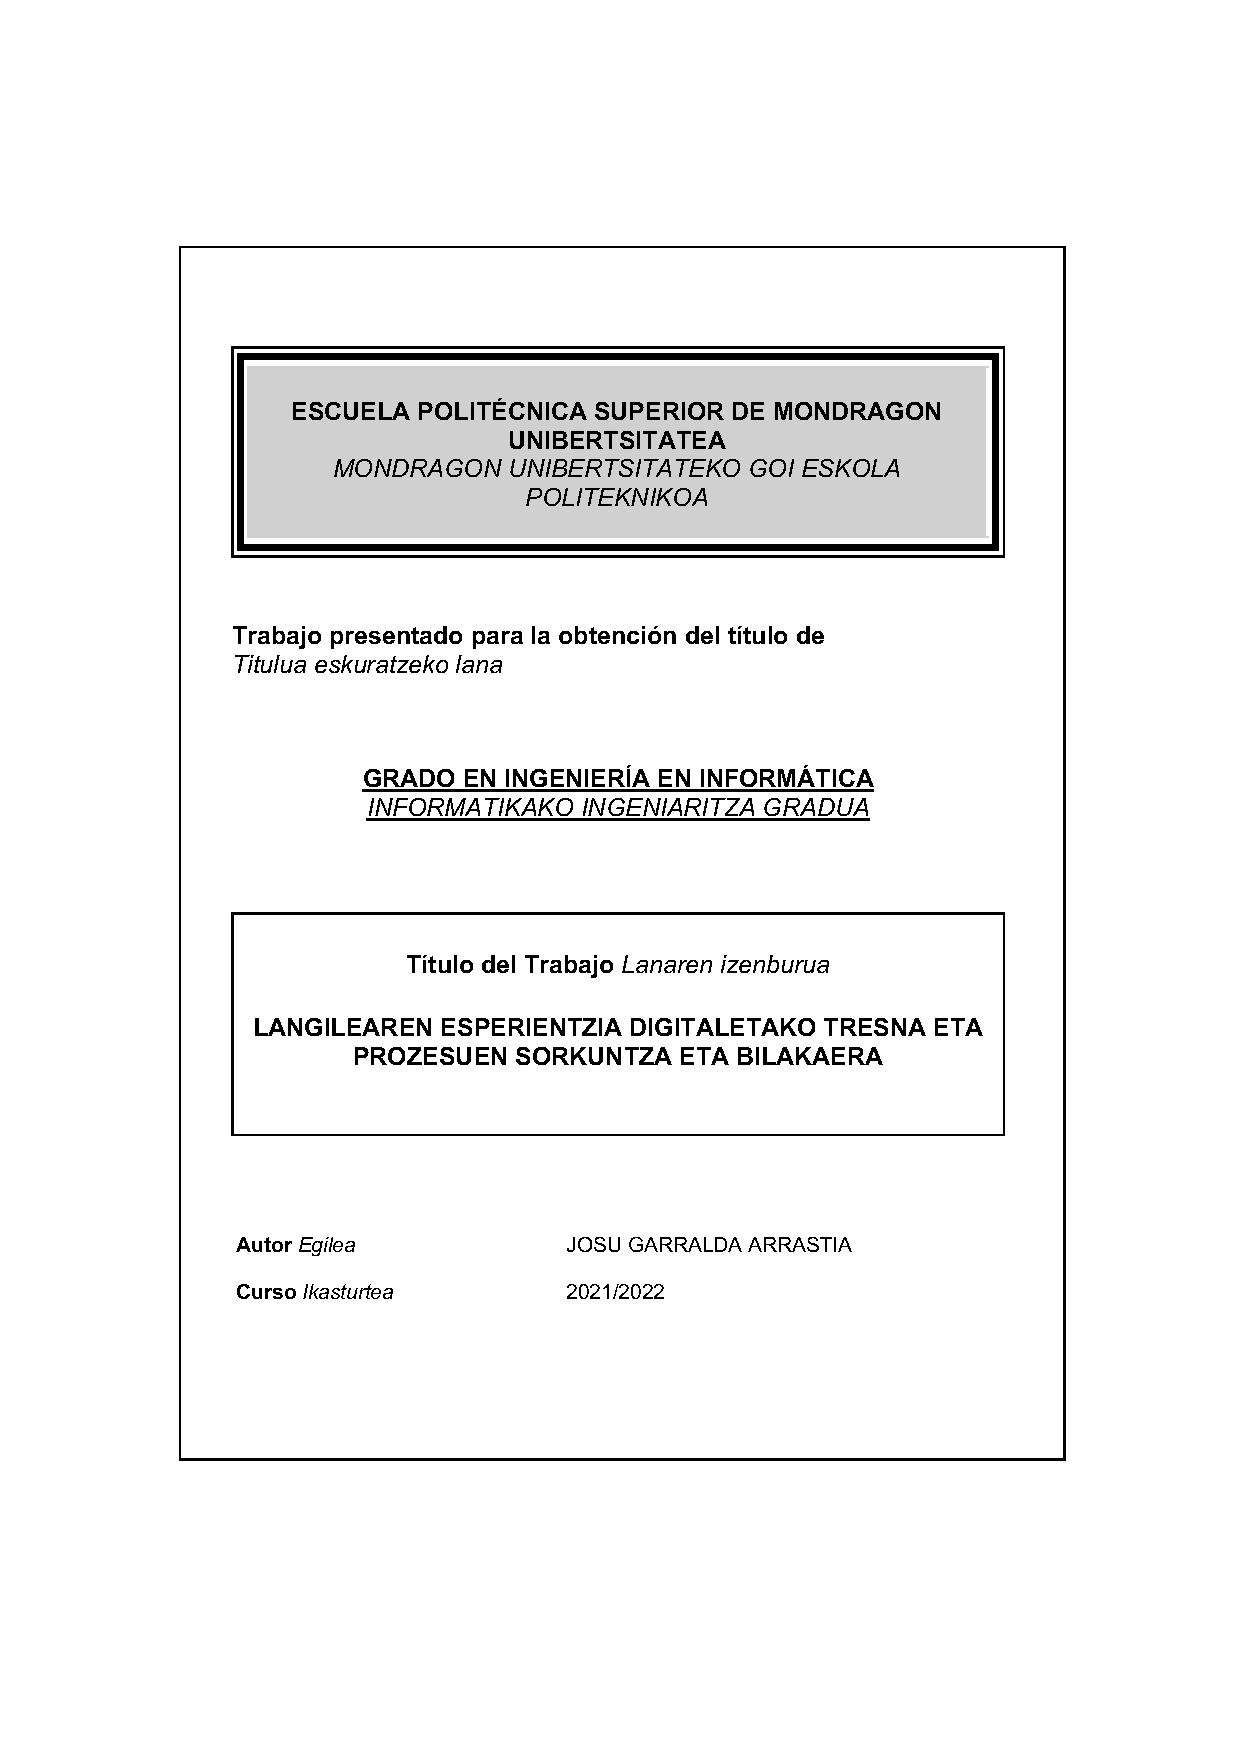
\includepdf[fitpaper=true, pages=-]{Assets/azala.pdf}

\newpage
\null
\thispagestyle{empty}
\newpage

  \chapter*{Agradecimientos}
En este documento en el que recojo el resultado del trabajo de fin de máster...

  \begin{center}
  {\Large \textsc{\textcolor{NavyBlue}{Abstract}}}
\end{center}
%
\noindent
%

\textsc{\textcolor{NavyBlue}{Keywords:}} 

\vspace{2cm}

\begin{center}
  {\Large \textsc{\textcolor{NavyBlue}{Resumen}}}
\end{center}
%
\noindent
%

\textsc{\textcolor{NavyBlue}{Palabras clave:}}
  \tableofcontents
  \listoffigures
  \listoftables

\mainmatter
  %%%%%%%%%%%%%%%%%%%%%%%%%%%%%%%%%%%%%%%%%%%%%%%%%%%%%%%%%%%%%%%%%%%%%%%%
\chapter{Sarrera}
%%%%%%%%%%%%%%%%%%%%%%%%%%%%%%%%%%%%%%%%%%%%%%%%%%%%%%%%%%%%%%%%%%%%%%%%


     Kapitulu honetan proiektua ulertu ahal izateko hainbat azalpen ematen dira. Alde batetik proiektuak soluzioa eman nahi dien arazoa azaltzen da, baita ere zein den industrian dauden ikuspegi ezberdinak honen inguruan. Bestetik proiektua garatzeko plangintza azaltzen da eta azkenik proiektua burutzeko beharrezkoa diren materiala eta baliabideak aurkezten dira baldintzen agirian.


%%%%%%%%%%%%%%%%%%%%%%%%%%%%%%%%%%%%%%%%%%%%%%%%%%%%%%%%%%%%%%%%%%%%%%%%
\section{Arazoa}
%%%%%%%%%%%%%%%%%%%%%%%%%%%%%%%%%%%%%%%%%%%%%%%%%%%%%%%%%%%%%%%%%%%%%%%%
Lan egiteko modua aldatu da, baita ere langileen espektatibak eta beharrak lan egiterako 
orduan. Langileek edozein lekutatik eta edozein gailutatik lan egin ahal izatea espero dute. 
Covid-19 pandemiak eragindako osasun larrialdiak, langileen kontziliazio beharrak eta telelanak lan ingurunea normaltasun berrira moldatzera behartu dute \cite{mckinsey-survey}.

Enpresentzak informazioaren antolakuntza, komunikazioa eta kolaborazioa beharrezkoa
dira eguneroko lanetan. 200 urtez erakundeek lantoki fisikoak eraiki dituzte,
ezagutu eta ulertzen ditugunak. Baina lanerako kontestuak izugarrizko eboluzioa bizi 
izan du eta orain lantoki digitalak, \emph{digital workplace} ere deituak, diseinatu eta hauei forma eman behar zaie. Plataforma hauek langileak, kolaboratzaileak eta bezeroak batzea lortzen dute.

Lantoki digitalen ikuspegiak lantoki fisikoen elementu guztien baliokideak jasotzen 
ditu: bileretarako, eztabaidetarako, produktibitaterako eta interakzio sozialetarako
tresnak esaterako. Lantoki digitalaren kontzeptuak ezagutzen ditugun intranetetatik
haratago doaz. Ez da proposatzen intranetak ''handitzea'' lantoki digital bihurtzeko, 
eboluzionatzea baizik mezularitza, bideo, kolaborazio tresnak eta aplikazioak gehituz.
Ikuspegi estrategikoa aldatu behar da eta intraneta lantoki digitalaren konponente bat 
bihurtzen da \cite{dwg-from-intranet-to-digital-workplace}.

Modu batean, aldaketa hauek onerako dira. Langileek, lanerako tresna egokiekin, edozeinekin eta edonondik lan egin dezakete. Edonondik lan egin ahal izatea da lantokien transformazioaren etorkizuna. Forrester-en arabera \cite{forrester-anywhere-work-strategy}, enpresen \%60ak lan egiteko modelo hibridoa erabiliko du aurrerantzean. Hau da, bulegoak eta lantegi fisikoak mantenduko dira baina edonondik lan egiteko aukera ere eskainiko da langileei. Honen helburua produktibitatearen onurak maximizatzea eta langileen asebetetze maila handitzea dira, lanerako hitzarmen malguen bitartez. Egoera berri honek erronka berriak dakartza negozioen liderrentzat.

Produktibitatearen inguruan, askok galdetzen diogu geure buruari ea nola den posible denok lanpetuta egotea eta era berean lanak aurrera egiten ez duela sentitzea. Lana aurrera eraman ahal izateko interakzio ezberdinak egiten ditugu, eta hauetako batzuk zentzurik ez dituztenean lana atzeratu egiten da. Lan eredu hibridorako bidean, interakzio asko aldatu, agertu edo desagertu daitezke. Trantsizio arrakastatsua lortzeko, interakzio hauek sailkatu eta aztertu behar dira ondoren soluzio teknologiko ezberdinetik eta automatizazioaren bitartez optimizatu ahal izateko \cite{mckinsey-interactions}.

Aldaketekiko erresistentzia handia egon daiteke hasiera batean bai zuzendarien artean, baita langileen artean ere. Produktibitate maila mantentzea, erakundearen kultura jarraitzea edo segurtasuna eta datuen pribatutasuna dira erronka esanguratsuenak. Erronkei aurre egiteko sormenezko irtenbideak behar dira. Komunikazio eta kolaborazio tresna bateratuak bezalako konponbide teknologikoek, sareko azpiegitura fidagarri eta seguruekin konbinatuta, oztopo horiek gainditzen lagun dezakete eta lantoki digitalak ahalbidetzen dituen aukerak maximizatzen.

Askorentzat ezaguna da Maslow piramidea \cite{wiki-maslow}, Abraham Maslow psikologoak garatutako gizakiaren motibazioei buruzko teoria. Teoria honek pertsonen beharrak premiaren arabera sailkatzen ditu. Piramidearen oinarrian behar fisiologikoak aurkitzen dira, bizitzeko ezinbestekoak direnak eta piramidean gorantz joan ahala beharren premia jaitsiz doa gailurrera iritsi arte, autoerrealizazioa.

Kontzeptu berdina jarrai dezakegu enpresaren beharrei erreparatuz, \ref{img:maslow} irudian azaltzen dena. Oinarrian kostuak murriztea eta irabaziak sortzea ditugu, gorago langile eta bezeroen asebetetzea eta azkenik tontorrean elkarlana, kultura berritzailea eta antolaketaren arintasuna ditugu.

\begin{figure}[h]
\centering
\includegraphics[width=0.7\textwidth]{Figures/sarrera/Maslows-Hierarchy-of-Enterprise-2.0-Needs.jpg}
\caption{Maslowren hierarkia enpresa ikuspegitik}
\label{img:maslow}
\end{figure}

Lantoki digitala ardatz da behar ezberdinak asetzeko. Kostuak murriztuz prozesu errepikakorrak automatizatuz, aukera berriei etekina ateraz, pertsonen nahiak betetzen dituzten soluzioekin edo kolaboratzeko tresnak martxan jarriz, besteak beste.

%%%%%%%%%%%%%%%%%%%%%%%%%%%%%%%%%%%%%%%%%%%%%%%%%%%%%%%%%%%%%%%%%%%%%%%%
\section{Aurrekariak eta artearen egoera}
%%%%%%%%%%%%%%%%%%%%%%%%%%%%%%%%%%%%%%%%%%%%%%%%%%%%%%%%%%%%%%%%%%%%%%%%

Eraldaketa digitala teknologia inplementatzeko eta honen onurak ustiatzeko enpresa batek hartzen dituen urrats eta ekintzak dira. Gaur egungo negozio-eragiketak
ulertuz hasten da prozesua eta teknologiaren bidez nola eboluzionatu daitezken
aztertzen da. 

Ezin da ahaztu transformazio digitalerako estrategiak hainbat saiakera, erabiltzaileen \textit{feedback}-saio eta denbora behar dutela emaitza positiboak lortzeko. Langile batzuentzat ''mundu digitalera'' trantsizionatzea erronka 
handia izan daiteke edo aldaketekiko erresistentzia erakusten dute. Konpainiek oztopo 
hauek gainditzeko plangintza sendo batekin erantzun behar dute. Maila eta mota 
guztietako langileen inplikazioa, liderren motibazioa eta lan-taldearen prestakuntza 
ezinbestekoak dira emaitza arrakastatsuak lortzeko. 

Azkeneko urteetako gertakariek telelana edo lan hibridoaren lan modalitatera moldatzera behartu ditu erakunde askori. Momentu honetan agerian gelditu dira enpresen plataformen gabeziak eta honen ondorioz langileentzako esperientziak sortzeko eskaera inoiz baino handiagoa da. 

Intranet plataformen egoera eta merkatua nola dagoen ezagutzeko Forrester agentziak argitaratutako \textit{The Forrester Wave™: Intranet Platforms, Q1 2022} txostena \cite{forrester-wave} hartu da erreferentzia modura. Txosten honetan intranet plataformak eskaintzen dituzten 12 enpresa eta produktu esanguratsuenak aztertzen dira: Akumina, Beezy, COYO, Igloo Software, Interact, LiveTiles, LumApps, MangoApps, Microsoft, Powell Software, Simpplr eta Unily. Enpresa hauen eskaintza, estrategia eta merkatu-tamaina konparatu dira talde ezberdinetan sailkatzeko: aurkariak, lehiakideak, lehiakide indartsuak eta liderrak. Geroz eta eskaintza eta estrategia sendoagoa izan, liderra izatetik geroz eta gertuago egongo da. 

Liderren artean Simpple, Unily eta LumApps daude. Hala ere, nahiz eta lehiakide indartsuen artean sailkatua egon, merkatuko presentzia altuena duen produktua Microsoften Microsoft 365 zerbitzua da. Izan ere, enpresek Microsoft aukeratzen dute \cite{why-companies-microsoft-365} jada ezagutzen dutelako, langileen gailuekin errez integratzen den plataforma osoa delako eta hodeiaren abantailak aprobetxatzen direlako. 

\newacronym{saas}{SaaS}{Software as a Service}

CYC (CYC CONSULTORIA Y COMUNICACIONES SI SL.)\footnote{CYC \url{https://www.cyc.es}} aholkularitza informatikoan aritzen den enpresa da, eraldaketa digitalerako soluzioetan aditua dena. Software aplikazioen eraikuntzan, datuen analisian, teknologiaren aplikazioa industrian eta intranet plataformen sorkuntzan lan egiten da, besteak beste. Modern Workplace eta Modern Workplace Evolution Services departamentuak dira langileentzako plataformen garapena eta jarraipena egiten dutenak eta helburu nagusia enpresetako komunikazioa hobetzea eta lan taldeen produktibitatea areagotzea da. Proiektu guztiek dute oinarri bera: Microsoften SharePoint eta Microsoft 365 \acrshort{saas} zerbitzua.

Microsoft 365 oinarri gisa erabiliz, honek eskaintzen dituen tresnak daude eskura: Office ofimatika \textit{suite} osoa, Outlook posta elektroniko zerbitzua, SharePoint guneak, Teams komunikazio eta kolaboraziorako aplikazioa... eta uneoro berrikuntzak gehitzen dira. Langilearen esperientziak hobetzeko asmoarekin 2021 urtean Viva\footnote{Microsoft Viva \url{https://www.microsoft.com/es-es/microsoft-viva}} tresna sorta aurkeztu zuen Microsoftek erakudeetan detektatu diren arazo ezberdinei erantzuna ematen dietenak: formakuntza, jakintzaren kudeaketa, osasun mentalaren zaintzea... Langileentzako plataformak eraikitzerako orduan, SharePoint guneak dira proiektu guztien oinarria eta guneen gainean konfigurazio eta garapen pertsonalizatuak inplementatzen dira. 

Plataforma hauen arrakasta areagotzeko eta langileei esperientzia intuitibo eta errazak eskaintzeko, gune eta tresnak pertsonalizatu behar dira kasu bakoitzaren kontestu eta egoerara egokituz. Pertsonalizatzeko aukerak anitzak dira: konfigurazio xume baten aldaketa egitetik, plataformaren barnean dagoen aplikazio oso baten eraikuntzara arte. Pertsonalizazio hauen eta eraikitzen diren guneetan dago plataformaren arrakastaren gakoa.  

SharePoint eta Teamsek eskaintzen duen esperientzia natiboa ez da aski izaten enpresen beharrak asetzeko, edo ez gutxienez modu eroso eta erabilgarrian egiteko. Erakundeek hamaika tresna erabiltzen dituzte normalean eta hauen arteko integrazioak ezinbestekoak izaten dira plataforma hauetan. 

%%%%%%%%%%%%%%%%%%%%%%%%%%%%%%%%%%%%%%%%%%%%%%%%%%%%%%%%%%%%%%%%%%%%%%%%
\section{Helburuak}\label{sec:helburuak}
%%%%%%%%%%%%%%%%%%%%%%%%%%%%%%%%%%%%%%%%%%%%%%%%%%%%%%%%%%%%%%%%%%%%%%%%
\newacronym{spo}{SPO}{Sharepoint Online}
Proiektuaren helburu nagusia beharrezko gai teknikoetan ahalduntzea da ondoren bezero errealentzako \acrfull{spo} eta Teamserako utilitateak eraiki ahal izateko. Soluzio hauek bezeroen beharrei erantzun behar diete eta bezeroen egoera zehatzetara egongo dira moldatuak.

Bestetik, departamentuaren parte bilakatzea eta departamentuko lanak bereganatzea da beste helburu nagusia. Helburu honen barne hainbat gaitasun lantzen dira: bezeroen arazoak eta egoera ulertzea eta hauei erantzuna emateko soluzioak sortzea, gerta daitezkeen dudei erantzuna ematea, akatsak araztu eta soluzionatzea, eta ingurune osoaren jarraipena egitea. 

%%%%%%%%%%%%%%%%%%%%%%%%%%%%%%%%%%%%%%%%%%%%%%%%%%%%%%%%%%%%%%%%%%%%%%%%
\section{Plangintza}
%%%%%%%%%%%%%%%%%%%%%%%%%%%%%%%%%%%%%%%%%%%%%%%%%%%%%%%%%%%%%%%%%%%%%%%%
Proiektuaren hasieran ez da emaitza zehatzik definitu, baina behin departamentuan integratzean ezagutuko dira egin beharreko atazak. Ataza hauek \ref{sec:helburuak} ataleko helburuak betetzeko balioko dute. 

Proiektuaren plangintza 2 faseetan banatzen da eta hurrengo lanak burutuko dira:
\begin{itemize}
    \item Microsoft 365ra orientatutako formakuntza
    \begin{itemize}
        \item Web garapena .NET, C\#, jQuery eta Kendu UI erabiliz. 
        \item SharePoint eta Teams pertsonalizatu SPFx, React eta TypeScript teknologiekin.
        \item PowerApps formulario pertsonalizatuak eta Power Automate ekintza automatikoak exekutatzeko fluxuak.
    \end{itemize}
    \item Modern Workplace Evolution Services departamentuan integratzea
    \begin{itemize}
        \item Bezero ezberdinentzako soluzioan diseinatu eta inplementatzea. 
        \item Microsoft 365en inguruko zerbitzua ematea: dudak argitzea eta erroreak konpontzea.
    \end{itemize}
\end{itemize}

Proiektuaren iraupen osoan zehar, honi dagokion txostena idatziko da.

Plangintza osoa eta hilabeteetan zehar egindako lanak \ref{app:gantt} eranskinean aurki daiteken Gantt diagraman irudikatu dira.

%%%%%%%%%%%%%%%%%%%%%%%%%%%%%%%%%%%%%%%%%%%%%%%%%%%%%%%%%%%%%%%%%%%%%%%%
\section{Baldintzen agiria}\label{sec:baldintzak}
%%%%%%%%%%%%%%%%%%%%%%%%%%%%%%%%%%%%%%%%%%%%%%%%%%%%%%%%%%%%%%%%%%%%%%%%
GBL proiektua zuzen garatzeko behar diren baliabide, betekizun eta baldintzak 
deskribatzen dira atal honetan. Garatuko den proiektua web 
teknologietan oinarritutako software tresna baten edo batzuen garapenean datza.

Sortutako soluzioa Microsoft SharePointen, Microsoft 365 ekosistemaren
barruan, oinarritutako aplikazioa, gune sorta edo konponentetaz osatuta egongo 
da. Gerta daiteke soluzioa Microsoft Teams plataformaren barruan egotea edo 
aurten merkaturatutako Viva aukerekin integratzea.

Produktua aurrera eramateko hurrengo puntuak bete behar dira:
\begin{itemize}
    \item Tresnak garatzeko behar diren teknologien formakuntza espezifikoa.
    \item Ordenagailua, pantaila eta bestelako osagarriak.
    \item Garapenerako ingurune osoa: Visual Studio, Visual Studio Code, Postman…
    \item Komunikaziorako plataforma: Microsoft Teams.
    \item Microsoft 365 harpidetza.
    \item Zalantzak eta bestelako ideiak komentatzeko lankidea(k).
    \item Eginbeharren arabera, gai edo eremu zehatzetan aditua den pertsona edo hauek kudeatzen dituena.
\end{itemize}

  %%%%%%%%%%%%%%%%%%%%%%%%%%%%%%%%%%%%%%%%%%%%%%%%%%%%%%%%%%%%%%%%%%%%%%%%
\chapter{Garapena eta emaitzak}
%%%%%%%%%%%%%%%%%%%%%%%%%%%%%%%%%%%%%%%%%%%%%%%%%%%%%%%%%%%%%%%%%%%%%%%%


     Kapitulu honetan proiektuan garatutako lanak eta lortutako emaitzak azaltzen dira. Emaitzetara iristeko garatutako lanen definizio funtzionala eta azalpen teknikoak deskribatuz, eta arrazoibidean fokua jarriz.



%%%%%%%%%%%%%%%%%%%%%%%%%%%%%%%%%%%%%%%%%%%%%%%%%%%%%%%%%%%%%%%%%%%%%%%%
\section{Atazen azalpena eta garatutako lanak}
%%%%%%%%%%%%%%%%%%%%%%%%%%%%%%%%%%%%%%%%%%%%%%%%%%%%%%%%%%%%%%%%%%%%%%%%
Praktiken garapenean zehar burututako ekintzak ezagutu eta ulertzea ezinbestekoa da lortutako emaitzak lortzeko prozesua ezagutzeko. 
\subsection{Formakuntza}\label{sec:bootcamp}
CYCn erabiltzen den \textit{stack} teknologikoa ezagutzeko, 3 hilabeteko \textit{bootcamp} motako formakuntza proposatu da
garapen inguruneak eta tresnak ezagutu, erabili eta barneratu ahal izateko. Formakuntza 6
kideko taldean burutu egin da, denok enpresan iritsi berriak. 3 zatitan banatu da formakuntza:
lehenik web teknologien oinarriak landu dira, ondoren Microsoft 365 ingurunean murgildu naiz
SharePoint eta Teams tresnetan fokua jarriz eta azkenik Microsoft Power Platformek
eskaintzen dituen Power Automate eta Power Apps \textit{no-code} edo \textit{low-code} tresnak landu dira soluzio
bizkorrak lortzeko. Prozesu honetan departamentu ezberdinetako kideak egon dira tutore
gisa. Atal bakoitza eduki teorikoekin hasi da, ondoren ariketa praktiko batean ikasitakoa
aplikatzeko eta azkenik beste kideekin eta tutorearekin berrikusi dira soluzio ezberdinak
aztertuz, tutoreen \textit{feedback}a lortzeko. 

\subsubsection{Web teknologiak: Frontend eta Backend}
Enpresan lantzen diren proiektu asko \textit{web}an oinarritutako soluzioak izaten dira. Soluzio
hauek eraikitzeko \textit{Frontend}ean HTML, CSS eta JavaScript hirukote ezaguna eta \textit{Backend}ean
Microsoften .NET \textit{framework}a C\# lengoaiarekin batera erabiltzen dira.

\textit{Frontend} aldearekin hasteko Pluralsight\footnote{Pluralsight \url{https://www.pluralsight.com}} ikasketarako plataformako hainbat ikastaro jarraitu
dira, honen oinarriak errepasatuz eta kontzeptu garrantzitsuenak bereganatuz. Ondoren, aplikazioen garapenaren departamentuko kide baten laguntzaz ariketa praktiko bat garatu da. 

Enpresa baten pertsonak eta egoitzak kudeatzeko tresna bat garatzea proposatu da. Alde batetik,
pertsonen zerrenda bat dugu eta bestetik egoitzen beste zerrenda bat, pertsona bakoitzak egoitza
bat erlazionaturik duela. Garatu beharreko soluzioak pertsonen eta egoitzen gainean CRUD
eragiketak (create-read-update-delete / sortu-irakurri-eguneratu-ezabatu) ahalbidetu behar ditu.
Soluzioa eraikitzeko .NET\footnote{.NET \url{https://docs.microsoft.com/eu-es/dotnet}} web proiektu bat sortuko da, Visual Studio\footnote{Visual Studio \url{https://visualstudio.microsoft.com/es/vs}} IDEa erabiliz, eta proiektu
hau oinarri harturik behar diren orrialdeak gehituko dira. Hasiera batean, pertsona eta 
egoitzen informazioa nabigatzaileko \textit{localstorage}ean gordeko da eta ondoren datuen persistentzia
datu base batean burutuko da. 

Soluzioaren itxura eta pantailen planteamendua guztiz librea da eta garapena azkartzeko Kendo UIk\footnote{Kendo UI \url{https://www.telerik.com/kendo-ui}}
eskaintzen dituen jQuery\footnote{jQuery \url{https://jquery.com}} konponente ezberdinak erabil daitezke. Nik planteatutako soluzioak, \ref{mecano1-table} irudian ikus daitekeena, orrialde
bakarra du eta orrialde honetan 2 taula daude pertsona eta egoitzekin. Taula batetik bestera nabigatzeko
goiko aldean bi botoi edo fitxa aurkitzen dira. 

\begin{figure}[H]
\centering
\includegraphics[width=0.9\textwidth]{Figures/garapena-emaitzak/formakuntza/mecano1-2/mecano1-1.png}
\caption{Pertsonak kudeatzeko taula nagusia}
\label{mecano1-table}
\end{figure}

Datuak nabigatzailearen \textit{localstorage}ko 2 \textit{array} modura gordetzen dira: bata pertsonekin eta bestea
egoitzekin. Pertsona bakoitzak erlazionatuta duen egoitza ezagutzeko pertsona batek ''EgoitzaId'' atributu
bat izango du. Egoitza bat ezabatu ahal izateko, ezin izango da egon pertsonarik egoitza honekin.

Pertsonak edo egoitzak sortzeko taula bakoitzaren gainean agertzen den ''Pertsona berria'' edo ''Egoitza
berria'' botoian sakatu beharko da. Leiho modal bat agertuko da datuak sartzeko formulario batekin, \ref{mecano1-modal} irudian ikus daitekena zehazki. Behin
datuak bete direla eta gordetzeko botoi sakatzean, datuak egiaztatu egiten dira eta datuak onargarriak badira
taulara gehituko dira. Datuak onargarriak ez badira, modalaren eremu ezberdinen azpian agertuko da
errore mezua. Taulako errenkada bakoitzean agertzen den ''Editatu'' botoia sakatzean modal  berdina
agertzen da. ''Ezabatu'' botoia sakatzean ordea, ezabatzea baieztatzea eskatzen da nabigatzaileko alerta
baten bidez.

\begin{figure}[H]
\centering
\includegraphics[width=0.9\textwidth]{Figures/garapena-emaitzak/formakuntza/mecano1-2/mecano1-EDIT.png}
\caption{Pertsona bat editatzeko leiho modala}
\label{mecano1-modal}
\end{figure}

Egoitza bat ezabatzeko orduan, egiaztapen gehigarri bat gertatzen da: pertsonarik ez egotea egoitza
honekin esleitua. Pertsonarik badago ezabatu nahi den egoitzarekin, eskuin-beheko ertzean errore mezu bat
agertuko da. Era berean, eragiketa arrakastatsu baten ondoren baieztapen mezu bat
agertuko da baita ere.

Behin soluzioa eraikita dagoela, datuak \textit{localstorage}tik datu base zentral batean gordetzera pasa da.
Aukeratutako datubasea Microsoften SQL Server\footnote{SQL Server \url{https://www.microsoft.com/en-us/sql-server}} da eta SQL Server Management Studio\footnote{SQL Server Management Studio \url{https://docs.microsoft.com/en-us/sql/ssms}} erabili da beharrezko
pertsonak eta egoitzak taulak sortzeko. Taula hauetako baten adibidea ikusten da \ref{img:sql-server} irudian. \textit{Frontend}aren eta datu basearen arteko komunikazioa ahalbidetzeko
\textit{REST API} web zerbitzu bat eraiki da. Datu basean prozedurak sortu dira web zerbitzuak burutu behar dituen
ekintzekin lotzeko eta CYCn erabiltzen den ORM (Object Relational Mapping) propioa erabili da. Web
zerbitzua garatzeko eta probatzeko Postman\footnote{Postman \url{https://www.postman.com}} erabili da. Postmanen bilduma bat sortu da dei guztiekin, \ref{img:postman} irudian agertzen den modura. Behin Postmanen dei guztien erantzunak nahi den
moduan jasotzean, \textit{Frontend}a aldatu egin da datuak datu basean gordetzeko \textit{localstorage}an egin ordez.

\begin{figure}[H]
\centering
\includegraphics[width=1\textwidth]{Figures/garapena-emaitzak/formakuntza/mecano1-2/mecano1-DB.png}
\caption{SQL Server-en sortutako taula, datuen persistentziarako}
\label{img:sql-server}
\end{figure}

\begin{figure}[H]
\centering
\includegraphics[width=1\textwidth]{Figures/garapena-emaitzak/formakuntza/mecano1-2/postman.png}
\caption{Postman bilduma, API-ak onartzen dituen deiak}
\label{img:postman}
\end{figure}

Edozein momentutan ere, web zerbitzuari egindako dei batek errore mezua itzultzen badu, erabiltzaileak
pantailan ikusiko du errore mezua. 

Lehen ariketa honen amaieran, pertsonak eta egoitzak kudeatzeko soluzio oso bat lortu da, datuak datu base
zentralizatu batean gordetzen dituena. Gainera, beste soluzio edo tresna batek pertsonen eta egoitzen
datuak eskuratu edo aldatu beharko balitu, garatutako web zerbitzua erabili daiteke.

\subsubsection{Microsoft 365, SharePoint eta SPFx}

CYCn, Modern Workplace departamentuan, Microsoft 365k eskaintzen duen inguruneaz baliatzen dira enpresa
ezberdinentzako langileen lantoki digitalak sortzeko. SharePointen oinarritutako soluzioak garatzen dira
gehienbat, Teams eta bestelako aplikazioekin integratzen direnak. Lehenengo urratsa Microsoft 365 eta
SharePoint ondo ezagutzean datza, ondoren SharePointek eskaintzen dituen funtzionalitate natiboak ezagutzeko
eta ondoren aukera eta pertsonalizazio berriak garatzeko. Erakunde batek SharePoint erabiltzean, gune ezberdinak
sor ditzazke. Gune hauek informazioa biltzen dute modu seguruan, guneko erabiltzaile baimenduek kontsultatu eta
aldatzeko aukera emanez. Guneetarako eta informaziorako sarbidea guztiz pertsonalizagarria da erabiltzaile eta taldeei
esleitzen zaien baimenen esker.

Erakundeek SharePoint bi modutan planteatu dezateke: bata SharePoint Server norberaren zerbitzarian \textit{on-premise}
moduan instalatuz eta bestea SharePoint Online SaaS moduko harpidetza kontratatuz. Gaur egun SharePoint Online
da aukeratuena, erakundeek ez dutelako zerbitzaririk mantendu behar eta Microsoft 365 harpidetzan barne dagoelako.
Harpidetza izanda Microsoftek garatutako azkeneko hobekuntza eta funtzionalitateak izango ditugu, Officeko
aplikazioak eta Teams komunikazio eta kolaboraziorako tresnak baita ere, besteak beste. 

Informazioa jasotzeko zerrendak edo dokumentu liburutegiak erabiltzen dira. Zerrendetan nahi haina
elementu sor daitezke, non elementu bakoitzak datu mota anitzeko propietateak edo atributuak izan ditzazke.
Dokumentu liburutegietan ordea, dokumentu ezberdinak jaso daitezke, soilik edo karpetetan bilduta. Zerrenda
elementuekin bezala, dokumentuek propietate ezberdinak izan ditzakete. Ikuspegi ezberdinak sor daitezke baita
ere, ikuspegi batean elementu edo dokumentu batentzat zein propietate eta zein ordenetan bistaratu nahi
diren aukeratu daiteke, baita elementuetan iragazkiak, taldekatzeak eta ordena ezarri ere.

Arestian aipatutakoa da SharePointek eskaintzen duen erabilera lehenetsia, baina badago aukera soluzio
pertsonalizatuak sortzeko, \acrfull{spfx} eta API ezberdinak erabiliz. 

\acrlong{spfx}, SharePoint guneetan soluzio pertsonalizatuak gehitzeko modua da, SharePointeko \textit{frontend}aren
garapenarekin bateragarritasun osoa du eta Teamseko funtzionalitatea zabaltzen du. Pertsonalizazio hauek 
JavaScript kodea injektatzen dute guneetan, React liburutegia erabiliz eta TypeScript lengoaian
idatzita daude. SharePointen edo Teams aplikazioan inplementatzen direnez, \textit{context}
izeneko objetu bat dute eskura. Objetu honi esker, soluzioaren kontestua eta APIak kontsumitzeko bezeroak
eskura daitezke. \acrshort{spfx} soluzio batean APIetara deiak egitean, soluzioa erabiltzen ari den
erabiltzailearekin autentikatzen dira. Horrela, soluzioaren erabiltzaileek bakarrik baimenduta dauden
ekintzak egin ahalko dituzte eta beharrezko informazioa besterik eskuratuko dute. 

SharePoint eta Microsoft 365ko datuekin lan egiteko SharePoint API eta Microsoft Graph API daude erabilgarri. SharePoint
APIaren bidez zerrendetako, dokumentu liburutegietako eta gune ezberdinetako informazioa eskuratu eta manipulatu daiteke.
Graph APIak ordea, SharePointeko informazioa eskuratuz aparte, Microsofteko beste tresnetako informazioa lortzen da.
Esaterako Direktorio Aktiboko erabiltzaileak eta taldeak, egutegiko bilerak, Teamseko elkarrizketak, Planneren
dauden eginkizunak... Graph APIa tresna berriagoa da SharePoint APIarekin alderatuz, eta SharePointeko datuak
lortzerako orduan SharePoint APIa Graph APIa baino osoagoa da. Hala ere, Graph APIak funtzionalitate gehiago ditu eta etorkizunera begira hau izango da erreferentziazko APIa.

Soluzio pertsonalizatuei begira, hainbat mota nagusi aurkitzen dira:
\begin{itemize}
  \item \textsb{Web zatiak}\footnote{SharePoint Framework - Web zatiak \url{https://docs.microsoft.com/sharepoint/dev/spfx/web-parts/overview-client-side-web-parts}}: SharePoint orrialde baten barnean agertzen diren kontrolak edo \acrshort{ui} elementuak dira eta
  nabigatzailean bertan exekutatzen dira. Web zatiak SharePoint Online-en orrialde bakarreko aplikazioak (\acrshort{spa}) edo
  Teamseko fitxak inplementatzeko erabil daitezke.
  \item \textsb{Aplikazio pertsonalizatzaileak}\footnote{SPFx luzapena - Aplikazio pertsonalizatzaileak \url{https://docs.microsoft.com/sharepoint/dev/spfx/extensions/get-started/using-page-placeholder-with-extensions}}: SharePoint guneetan goiburu eta orri-oinak pertsonalizatzen dituzte.
  \item \textsb{Eremu pertsonalizatzaileak}\footnote{SPFx luzapena - Eremu pertsonalizatzaileak \url{https://docs.microsoft.com/sharepoint/dev/spfx/extensions/get-started/building-simple-field-customizer}}: Zerrenda edo dokumentuen liburutegi batean eremu baten itxura eta formatu
  lehenetsia aldatzen dute.
  \item \textsb{ListView komando multzo luzapenak}\footnote{SPFx luzapena - ListView komando multzo luzapenak \url{https://docs.microsoft.com/sharepoint/dev/spfx/extensions/get-started/building-simple-cmdset-with-dialog-api}}: luzapen hauek zerrenda edo dokumentu liburutegi batean ekintza berriak
  gehitzea ahalbidetzen du. Ekintza berri hauek elementu batek duen komando baten bidez abiarazten dira. 
  \item \textsb{Bilaketa luzapenak}\footnote{SharePoint Framework - Bilaketa luzapenak \url{https://docs.microsoft.com/sharepoint/dev/spfx/building-search-extensions}}: Bilaketa bat exekutatu aurretik bilaketaren edukia aldatzeko balio dute. Oraingoz, aurrebistan daude eta gutxien hedatu den pertsonalizazio mota da.
\end{itemize}

Soluzioak eraikitzerako orduan, SharePoint-en diseinu eta \textit{look and feel} berdinak jarraitzeko
Fluent UI\footnote{Fluent UI \url{https://developer.microsoft.com/en-us/fluentui}} Microsoften diseinu sistema erabiltzea oso gomendagarria da.
Fluent UIk React konponente ezberdinak eskaintzen ditu, diseinu eta erabiltzailearen esperientziaren aldetik SharePointen guztiz
bat egiten dutenak eta SharePointeko esperientzia natiboarekin konparatuz berdina dena. Konponenteak eskaintzean gain, hainbat diseinu
jarraipen ematen dira, baita garapenetan erabili daitezken ikono sortak ere. Fluent UIren helburua da erabiltzaileen esperientzia eta
itxura koherentea izatea Microsoft 365 produktuaren osotasunean. 

Aipatzekoa da baita ere Microsoft 365 garaperaren inguruan dagoen komunitatea. Komunitate honek SharePoint, Teams eta Microsoften API
ezberdinetarako soluzio libre eta berrerabilgarriak eraiki eta mantentzen ditu. Komunitate esanguratsuena
\acrfull{pnp}\footnote{\acrfull{pnp} \url{https://pnp.github.io}} da 
eta Microsoften langilez eta beste garatzailez osatua dagoen \textit{open-source} ekimena da.
Komunitatearen xedea garapen dokumentazioan, soluzio adibideetan, eta Microsoft 365en erabilera eta garapenari buruzko ekimenetan
ekarpenak egitea da. 

Hurrengoak dira \acrshort{pnp} komunitateak sortu dituen tresna eta \acrshort{sdk} erabilgarrienak:
\begin{itemize}
  \item \textsb{PnP SPFx Yeoman Generator eta Teams Yeoman Generator}\footnote{PnP Yeoman Generator \url{https://pnp.github.io/generator-spfx}}: SPFx eta Teamserako soluzioen proiektuek egitura zehatz bat izan
  behar dute eta egitura hau modu errezean sortzeko tresna hau erabiltzen da. Garatu beharreko web zati edo luzapenaren arabera sortzen du
  proiektuaren egitura, \textit{scaffolding} edo aldamio izenaz ezaguna. 
  \item \textsb{PnPjs liburutegi multzoa}\footnote{PnPjs \url{https://pnp.github.io/pnpjs}}: SharePoint, Graph eta Microsoft 365 APIak kontsumitzeko liburutegiak eskeintzen ditu.
  TypeScript-erako datu motak erabiltzearen abaila du, honek dakarren segurtasuna aprobetxatuz. 
  \item \textsb{SharePoint Framework reusable React controls}\footnote{PnP SPFx reausable React controls \url{https://pnp.github.io/sp-dev-fx-controls-react}}: biltegi honek React kontrol bererabilgarriak eskeintzen ditu. Kontrol
  hauek \acrshort{spfx} web zati eta luzapenetan erabil daitezke. Kontrol hauek Fluent UI diseinu sistema jarraitzen dute. 
  \item \textsb{SharePoint Framework reusable property pane controls}\footnote{PnP SPFx reusable property pane controls \url{https://pnp.github.io/sp-dev-fx-property-controls}}: biltegi honek \acrshort{spfx} soluzio bat konfiguratzeko
  erabiltzen den propietate panelerako kontrol ezberdinak eskaintzen ditu. Kontrol hauek Fluent UI diseinu sistema jarraitzen dute.
\end{itemize}

Tresna hauei esker garapen denbora eta konplexutasuna murriztu egiten dira eta garatzaileok eskura ditugun tresna eta liburutegi hauek
konbinatzen dira emaitza egokiak lortzeko.

SPFx soluzio moten artean gehien erabiltzen dena web zatia da, eta horregatik proposatutako praktikarako ariketa web zati bat garatzean
datza, SharePoint API eta Graph APIak kontsumitzen dutenak.

Praktikarako ariketaren helburua albiste ezberdinak bistaratzen dituen web
zati bat da. \ref{ads-template} irudian ikus daiteke soluzioaren kontzeptua. Zerrenda batean albisteak jasoko dira hainbat propietaterekin batera: irudia, deskribapena, kategoria... Web zatian
albisteak txarteletan bistaratuko dira eta txartelean klik egitean leiho modal bat agertuko da albistearen informazio osoa eta albistearen
argitaratzailearen kontakturako informazioa erakutsiz. Albisteak iragazi egin ahalko dira kategoriaren arabera eta emaitza guztien
kontagailu bat agertu behar da. Web zatia erabiltzailearen pantailaren tamainara egokitu behar da, \textit{responsive} diseinua erabiliz.
Web zatia erakusteko konfiguratu egin behar da, era erraz batean web zatiak erakusten dituen iragarkien zerrenda aukeratuz. 

Soluzioa eraikitzerako orduan, aurreko betekizunez gain hainbat hobekuntza gehitu dira: emaitzen orrikatzea, emaitzak \textit{cache}
modura gordetzea eta web zatia hizkuntza deberdinetara itzultzea.

Web zatia orrialde batera gehitzean, hau konfiguratzeko mezua agertuko da pantailan, \ref{ads-configuration} irudian bezala. Konfiguratu botoia sakatzean, alboko panel batean
konfiguragarriak diren propietateak aukera daitezke: iragarkiak dituen zerrenda, emaitzen orri bakoitzean agertzen diren iragarki
kopurua eta irudirik ez duten iragarkietan agertu behar den lehenetsitako irudiaren URLa. Propietate hauek aldatzeko erabiltzen diren
kontrolak SharePoint Framework Reusable Property Pane Controls biltegitik lortu dira. Zerrenda aukeratzeko kontrolak automatikoki
lortzen ditu web zatia jarrita dagoen gunean dauden zerrendak, erabiltzaileak bat aukera dezan. Orriko elementu kopurua eta lehenetsitako
irudiaren eremuak ordea, Fluent UIk eskainitako kontrolekin eraiki da. Soluzio osoan erabilitako Fluent UIren kontrolek SharePoint gunearen
kolore paleta erabiltzen dute.

\begin{figure}[H]
\centering
\includegraphics[width=0.9\textwidth]{Figures/garapena-emaitzak/formakuntza/iragarkiak-web-zatia/mecano3-azalpena1.png}
\caption{Proposatutako ariketaren eskema bisuala}
\label{ads-template}
\end{figure}

\begin{figure}[H]
\centering
\includegraphics[width=0.9\textwidth]{Figures/garapena-emaitzak/formakuntza/iragarkiak-web-zatia/mecano3-emaitza-konfiguratu.png}
\caption{Web zatia konfiguratzeko ezarpenak}
\label{ads-configuration}
\end{figure}

Behin web zatia konfiguratuta dagoela, SharePoint APIa erabili da iragarkiak lortzeko. Hasiera batean, web zatia konfiguratzean
ezarritako iragarki kopurua kargatuko da eta iragarki gehiago badaude kargatzear, azpiko aldean hurrengo iragarkiak kargatzeko
botoia agertuko da. Kontrako kasuan, iragarki guztiak kargatu direla jakinaraziko du. Goiko aldean, ezkerreko aldean iragarki kopuru
totala agertuko da. Ezkerraldean, iragarkiak kategoriaren arabera iragazteko kontrola. Emaitzak erakusten diren gunea, erabiltzailearen
pantaila edo leihoaren zabalerara moldatzen da (ikus \ref{ads-responsive} irudia): gailu txikienetan zutabe bakarrean erakutsiz, ertainetan bitan eta zabalenetan hirutan. 

\begin{figure}[H]
\centering
\includegraphics[width=1\textwidth]{Figures/garapena-emaitzak/formakuntza/iragarkiak-web-zatia/iragarkiakwebzatia1.png}
\caption{Iragarkien web zatia, pantaila tamaina ezberdinetan.}
\label{ads-responsive}
\end{figure}

Erabiltzaileen esperientzian pentsatuz, soluzioak erakusteko iragarkirik ez duen egoeran pentsatu da. Egoera hutsean, alegia. Iragarkien
zerrendan iragarkirik ez badaude, mezu bat agertzen da egoera azalduz eta emaitzak lortzeko gomendioak emanez. \ref{ads-empty} irudian ikus daiteke egoera hau.

\begin{figure}[H]
\centering
\includegraphics[width=0.8\textwidth]{Figures/garapena-emaitzak/formakuntza/iragarkiak-web-zatia/mecano3-zerrendahutsa.png}
\caption{Iragarkien web zatia, egoera hutsean.}
\label{ads-empty}
\end{figure}

Iragarkien txartel batean klik eginez, iragarkiaren informazio osoa agertzen da \ref{ads-modal} irudiko leiho modalean bezala. Iragarkiaren informazioaz aparte,
iragarkia argitaratu den kontakturako datuak eta momentuko eskuragarritasuna ikusiko ditu erabiltzaileak. Iragarkia argitaratu duen
pertsonaren datuak Graph APIa erabiliz lortu dira, erabiltzailearen informazioa  eta erabilgarritasuna ''users'' eta 
''presence'' \textit{endpoint}etatik lortu da, hurrenez hurren.

\begin{figure}[H]
\centering
\includegraphics[width=1\textwidth]{Figures/garapena-emaitzak/formakuntza/iragarkiak-web-zatia/mecano3-modal.png}
\caption{Iragarki baten informazio osoa, leiho modalean.}
\label{ads-modal}
\end{figure}

Soluzioan zehar, web zatiaren errendimendua eta APIetara egiten diren deiak minimizatzeko APIetatik lortzen diren datuak denbora batez
nabigatzaileko \textit{local storage}an gordetzea erabaki da. Honen adibidea \ref{ads-caching} irudian agertzen da. Prozesu hau errazteko 
PnPClientStorage\footnote{PnPClientStorage \url{https://pnp.github.io/pnpjs/core/storage/}} modulua erabili da.
Web zatian zehar Sharepoint APItik iragarkien datuak lortzen dira eta Graph APIaren bitartez erabiltzaileen informazioa eta eskuragarritasuna.
Iragarkien eta erabiltzaileen informazioa gorde egiten da, baina eskuragarritasuna uneoro alda daitekenez, iragarki txartel bat irekitzen den
bakoitzean eskuragarritasuna eskatuko zaio Graph APIari.

\begin{figure}[H]
\centering
\includegraphics[width=1\textwidth]{Figures/garapena-emaitzak/formakuntza/iragarkiak-web-zatia/mecano3-caching.png}
\caption{Nabigatzaileko \textit{local storage}a, APIetako erantzunekin.}
\label{ads-caching}
\end{figure}


\subsubsection{Microsoft Power Platform}
Microsoft Power Platform\footnote{Microsoft Power Platform \url{https://powerplatform.microsoft.com}} \textit{business intelligence}, aplikazioen garapen eta automatizaziorako software sorta da. Erabiltzaile
ez-espezializatuei dago orientatua eta aplikazio eta automatismoak sortzeko web tresnak eskaintzen ditu. Power Platformaren
arteko logika adierazteko Microsoftek Power Fx\footnote{Microsoft Power Fx \url{https://docs.microsoft.com/en-us/power-platform/power-fx/overview}} \textit{low-code} programazio lengoaia garatu du. Datu jatorri ezbedinetako informazioa erabili
eta manipula daiteke integrazio eta kontektoreen bidez. Excel, CSV fitxategiak, SQL datubaseak dira datu jatorrietako batzuk, eta
SharePoint eta web zerbitzuekin integra ditzazkegu sortutako soluzioak.

Hauek dira Power Platform familiak dituen produktuak:

\begin{itemize}
  \item \textsb{Power BI}\footnote{Power BI \url{https://powerplatform.microsoft.com/en-us/power-bi}}: datuak bisualizatzeko eta analizatzeko softwarea. Datu hauen analisiari esker erakundeei erabakiak hartzea
  laguntzen dute.
  \item \textsb{Power Apps}\footnote{Power Apps \url{https://powerplatform.microsoft.com/en-us/power-apps}}: negozio beharrak asetzeko \textit{low-code} aplikazio pertsonalizatuak eraikitzeko software grafikoa. Aplikazio
  independienteak, SharePointen bertan txertatu daitezkeenak, eta SharePointeko formulario ezberdinak pertsonaliza daitezke baita ere.
  \item \textsb{Power Automate}\footnote{Power Automate \url{https://powerplatform.microsoft.com/en-us/power-automate}}: lan fluxuak inplementatzeko tresna. Gertakari baten ondoren exekutatu behar diren ekintzak automatizatzen
  laguntzen du.
  \item \textsb{Power Virtual Agents}\footnote{Power Virtual Agents \url{https://powerplatform.microsoft.com/en-us/power-virtual-agents}}: chatbot adinmendunak eraiki eta inplementatzeko tresna.
\end{itemize}

Gauden kontestua  kontuan hartuta, Power Apps eta Power Automate tresnak erabiltzen dira. Datu jatorri bezela SharePointeko
zerrendak eta dokumentuen liburutegiak izango ditugu.

Power Appsen bidez zerrendetako elementuen formularioak pertsonalizatu daitezke. SharePointeko lehenetsitako
formularioekin alderatuz Power Appsi esker formularioan agertzen diren eremuak, hauen posizioa eta itxura alda daiteke. Nahi izanez gero
botoiak, irudiak, taulak eta bestelako kontrolak gehi daitezke. Formularioen kasuetarako interesgarria den beste funtzionalitate bat APIetarako
deiena da. Eremu bat balidatzeko edo eremu baten duen balioaren arabera beste eremu batzuk dete daitezke web zerbitzu baten emaitza erabiliz.
Formularioko eremua aukera motakoa denean, aukera daitezken balioak web zerbitzu bati esker lor daitezke ere. 

Power Automate-i esker, SharePointeko zerrenda ezberdinetako gertakarien ondoren hainbat ekintza automatiza daitezke: jakinarazpenak bidaltzea,
elementu berriak sortzea edo elementuen gaineko baimenak aldatzea, besteak beste. Gertakari baten ondoren exekutatu behar den fluxu bat
diseinatzen da. Fluxu hauek funtzio baten modura trata ditzazkegu: aldagaiak sortuz, baldintzak eta begiztak gehituz, salbuespenak tratatuz...

Proposatutako praktikaren helburua erakunde batean egindako gastuen jarraipena burutzea da. Jarraipen honetan erabiltzaileek gastuaren inguruko
informazioa emango dute eta arduradun ezberdinek gastu hauek balidatuko dituzte. Gastu bakoitzak erlazionatutako egin behar bar izango du.
Prozesu guztian zehar posta elektronikoz gastuaren inguruko zehetasunak eta eguneraketak jakinaraziko dira. Garrantzia eman zaio datuen segurtasunari eta hauen gaineko baimenei. 

Soluzioaren oinarrizko egitura erreparatuz 3 zerrenda ditugu:

\begin{itemize}
  \item \textsb{Gastuak}: prozesuaren oinarrizko elementua da. Zerrenda honetako elementuek gastuaren inguruko informazio guztia jasoko
  dute: gastuaren izena, deskribapena, prezioa, dagokion departamentua, egoera eta dokumentu erantsiak. Gastu bat zirriborro moduan gorde daiteke,
  ''Balidatzera bidali'' bai/ez eremu bati esker. Eremu hau baiezkoarekin bidaltzen bada, dagokion departamentuko arduradunak jasoko du
  eskaera eta erabiltzaileak ezin izango ditu aldaketak egin gastuan.
  \item \textsb{Departamentuak}: Erakundeko departamentu ezberdinak eta bakoitzaren arduradunak jasotzen dira zerrenda honetan. Zerrenda
  honetako departamentuak, gastuen zerrendako departamentuko aukerak dira. Arduradunen informazioa jakinarazpenak bidaltzeko erabiliko da.
  \item \textsb{Zereginak}: gastu bakoitzak zeregin bat izango du. Zereginaren datu gehienak gastuaren informazioarekin beteko dira (izenburua,
  balidatzaileak eta eranskinak esaterako), eta erabiltzaileak ezingo du zuzenean zeregin elementurik sortu. Balidatzaileek egoera eta
  baztertzeko arrazoia eremuak beteko dituzte zeregin bakoitzerako.
\end{itemize}

Alde batetik, Power Apps erabili da zerrendetako formularioak pertsonalizatzeko: elementu berria sortzeko, elementuak ikuskatzeko eta
editatzeko formularioak. Gastuen zerrendan formularioak gastuaren egoerara moldatu dira, beharrezko eremuak bakarrik erakutsiz eta aldatu ez daitezkeen
eremuak ezkutatuz edo irakurketarako bakarrik mugatuz. Atazen formularioetan ordea, elementu berria sortzeko formularioa hutsik utzi da. Zeregin berria
sortzeko formularioan mezu bat agertzen da esanez lehendabizi gastu bat sortu beharko duela, eta gastu hau sortzeko formulariora daraman botoi bat
agertzen da. Gastuekin gertatzen den bezala, zeregin baten egoeraren arabera formularioko eremuak aldatzen dira.

Bestetik, Power Automate erabili da gastuari dagokion zeregina sortzeko, elementuen gaineko baimenak aldatzeko eta erabiltzaileei jakinarazpenak
bidaltzeko:

\begin{itemize}
  \item Gastu bat balidatzera bidaltzean, zeregin berri bat sortuko da gastuaren datuekin eta gastuaren departamentuko balidatzaileei jakinaraziko zaie
  posta elektroniko bidez gastu eta zeregin berri hauetaz. Gastua sortu duen erabiltzaileak gastua bera eta honi erlazionatutako zeregin ikusi ahalko ditu
  soilik. Gastuaren balidatzaileek ordea, gastua ikusteko eta zeregina editatzeko baimena izango dute. 
  \item Balidatzaile batek zeregin bat editatzean eta honen egoera aldatzean: dagokion gastuaren egoera eguneratuko du, gastuaren eta zereginaren baimenak
  aldatuko ditu eta gastuaren sortzailea jakinaraziko du posta elektronikoz.
\end{itemize}

Praktika honetan egindakoa Power Platformen erabilera kasu bat da, baina plataformak dituen aukerak infinituak dira. Power Apps aplikazio osoak eraikitzeko
erabil dezakegu. Erabiltzaileekin interaktuatzeko pantaila ezberdinak sortuz eta datu iturri anitzetara konektatuz, modu arin batean lortzen dugu negozio
beharrak asetzen dituen aplikazio bat sortzea. 

Power Automatek exekutatu ditzazken ekintzak ere denetarikoak dira: fitxategien manipulazioa, deiak web 
zerbitzuetara, Microsoften tresna ezberdinekiko integrazioak... Gainera, aukera natiboek ez dituztenean beharrak guztiz betetzen Power Appsen
Power Component Framework (PCF)\footnote{Power Components Framework \url{https://docs.microsoft.com/en-us/power-platform/alm/component-framework}} kontrolak sor daitezke, HTML, CSS, JavaScript eta React erabiliz edo Power Automaterako konektore pertsonalizatuak baita ere.

\subsection{SPFx soluzioen analisia SonarQube bidez} \label{sonarqube}

Modern Workplace eta Modern Workplace Evolution Services departamentuetan SPFx motako soluzioak eraikitzea ohikoa da.
Soluzio hauen kalitatea neurtzeko SonarQube\footnote{SonarQube \url{https://www.sonarqube.org}} tresna erabili nahi da. CYCko beste departamentuan jada martxan dago eta honen erabilera hedatu nahi da gainontzeko departamentuetara.
Helburua SPFx motako proiektuak analizatzea da, kalitate profil pertsonalizatu bat sortuz. Proiektuen analisirako beharrezko pausu eta argibideak dokumentu batean jaso dira. SonarQube erabiltzeko beharrezkoak diren pausuak, konfigurazioak eta konponente ezberdinen probak Asier Aldekoa lankidearen batera garatu da. 

SonarQube SonarSource\footnote{SonarSource \url{https://www.sonarsource.com}} enpresak garatutako plataforma da; kodearen kalitatea ikuskatzen duena honen analisi estatikoa burutuz. Analisiaren emaitzan bikoiztutako kodea, kodetzeko estandarren jarraipena, konplexutasuna eta segurtasun-gomendioak ematen dira. Tresna honi esker, kodearen kalitatea neur daiteke proiektuaren osotasunean. 

SPFx proiektuek TypeScript lengoaian daude idatzita ia osotasunean baina JavaScript eta SCSS fitxategiak ere izan ditzakete. Analisia burutzerako momentuan
SonarQubek lengoaia hauek detektatuko ditu eta zerbitzarian lengoaia hauentzako ezarritako kalitate profilak aplikatuko ditu.

Konponente berri bat sortzerakoan, SonarQube zerbitzarian proiektu berri bat sortu beharko da.
Proiektu honek TypeScript lengoaiarentzat sortutako ''CYC Profile'' deituriko profila jarraituko du.
Profil hau ''Sonar way recommended'' lehenetsitako profiletik eratorria da eta denborak aurrera egin ahala eta analisiek emandako emaitzak kontuan hartuta eboluzionatzen joango da.
Bestetik, erakunde osoan erabiltzen den ''CYC Quality Gate'' kalitate baldintzak kontuan hartzen dira proiektu batek analisia gainditzen duen ala ez kalkulatzeko.

Kodearen analisia eta kalitate arazoak garapen ingurumean bertan burutzeko eta ezagutzeko SonarLint\footnote{SonarLint \url{https://www.sonarlint.org}} Visual Studio Code kode-editorearentzako luzapena erabili da.
SonarLint konfiguratu da zerbitzaritik proiektuaren kalitate profila detektatzeko eta honetan ezarritako erregelak analisian aplikatzeko.
Luzapen honi esker kodearen analisia exekutatzen da lokalean eta analisian aurkitutako arazoak, beste errore eta abisuekin batera agertzen dira.
Lokalean egindako analisiaren emaitzak ez dira zerbitzariko analisiarenak bezain osoak, baina kodea garatzeko momentuan bertan abisuak jasotzea abantaila handia da. \ref{img:sonarlint} irudian ikus daiteke nola erakusten den SonarLinten analisiaren emaitza Visual Studio Code kode-editorean. 

Zerbitzarian analisia egiteko, \textit{sonar-scanner} komando lerrorako tresna erabili da.
Analizatu nahi diren proiektuetan jada \textit{sonar-project-properties} fitxategi bat egongo da proiektuaren gakoa eta SonarQube zerbitzariaren informazioarekin, beste informaziorekin batera.
Proiektuaren errotik \textit{sonar-scanner} komandoa exekutatzeko nahikoa izango da erabiltzailearen segurtasun tokena jartzea. 

\begin{figure}[H]
\centering
\includegraphics[width=1\textwidth]{Figures/garapena-emaitzak/sonarqube/sonarlint.png}
\caption{SonarLint luzapenak egindako analisiaren emaitzak Visual Studio Coden}
\label{img:sonarlint}
\end{figure}

Modern Workplace departamentuak SPFx konponente ezberdinak garatuta ditu, bezero ezberdinen proiektuetan erabiltzen direnak.
Proba modura, eta analisiaren emaitzak ematen dituen abisuak ezagutzeko konponente batzuk analizatu dira. \ref{img:sonarqube-analisia} irudian ikus daiteke adibide bat. 

\begin{figure}[H]
\centering
\includegraphics[width=1\textwidth]{Figures/garapena-emaitzak/sonarqube/sonarqube-server.png}
\caption{UserProfileViewer SPFx soluzioaren analisiaren emaitzak}
\label{img:sonarqube-analisia}
\end{figure}

Hainbat proiektu analizatu ondoren \ref{table:sq-analisia-emaitzak} taulako ondorengo abisuak dira ohikoenak:
\begin{table}[ht]
\centering
\rowcolors{2}{teal!0}{teal!10}
\def\arraystretch{1.5}%
\begin{tabular}{ p{9cm} p{2.25cm} p{2.25cm}  }
\hline
\textbf{Arazoa} & \textbf{Mota} & \textbf{Larritasuna} \\
\hline
''forEach'' funtzioa erabili ''map'' ordez, funtzioak itzulitako balioa erabiltzen ez denean.  & Bug & Baxua \\
Aldatzen ez diren aldagaiak ''const'' batez hasieratu behar dira. & Code smell   & Kritikoa \\
Funtzio baten konplexutasun kognitiboa 15 izan daiteke gehienez.  & Code smell & Kritikoa \\
Funtzio eraikitzailean bakarrik esleitzen diren propietate pribatuak ''readonly'' erabiliz deklaratu behar dira. & Code Smell& Altua \\
Ezin dira komentatuako kode zatiak egon. & Code smell & Altua \\
Adierazpenak lerro ezberdinetan egon behar dute. & Code smell & Altua   \\
''==='' eta ''!=='' erabili behar da ''=='' eta ''!='' ordez. & Code smell & Altua \\
Fitxategiek amaieran lerro huts bat eduki behar dute. & Code smell & Baxua \\
\hline
\end{tabular}
\caption{SonarQube analisietan aurkitutako arazo ohikoenak}
\label{table:sq-analisia-emaitzak}
\end{table}

Kasu bakoitzeko arazoak aztertu eta zuzenduko dira. Positibo faltsu edo erantzuna eman nahi ez zaien arazoak baloratuko dira kalitate profileko erregelak aldatzeko. Era berean, garatzaile taldeak adostuko du zein erregela gehitu edo kendu behar diren etorkizuneko proiektuei begira.

\subsection{Iradokizunak jasotzeko eta kudeatzeko soluzioa}\label{sec:iradokizunak}
Modern Workplace departamentuak SharePoint eta Teamsen oinarritutako lan ingurune digitala eraiki du bezero batentzat. Bezeroak orain arte SharePoint Server
2007n oinarritutako intraneta du, baina Microsoft 365 eta hodeiaz baliatu nahi dute lankideen arteko komunikazioa eta kolaborazioa hobetzeko. Bezeroak industriaren
sektorean lan egiten du. Egoitza nagusia Euskal Autonomia Erkidegoan du, baina baditu beste egoitza batzuk nazioartean. Ondorioz, ingurune digitala 6 hizkuntzatan
dago eskuragarri. Orain arte erabili duten intranetean, badaude hainbat zerbitzu eta gune langileen eskura daudenak eta hauek ingurune berrira migratu behar dira.

\subsubsection{Abiapuntua eta beharren analisia}
Bezeroak langileen iradokizunak jasotzeko sistema du inplementatuta, SharePoint zerrendetan oinarritua.
Iradokizun hauen xedea produktu eta prozesuen hobekuntza lortzea da; kalitate, errentagarritasun, eraginkortasun eta ingurumen aldetik. 

Gune honetan langileek iradokizun berri bat sortu dezakete formulario bat betez,
proposatutako egoera azalduz eta iradokizunaren inguruko ebidentziak edo irudiak erantsiz. Aipatzekoa da plantako langileek,
Microsoft 365 konturik gabekoak, iradokizun hauek paperezko formulario bat betez egiten dituztela. 
Iradokizuna jaso ondoren kalitateko arduradun batek iradokizuna sailkatu eta iradokizuna kudeatzeko arduradun bat esleituko dio.
Arduradun honek proposatutako egoerara iristeko ekintza batzuk deskribatuko ditu eta iradokizunaren jarraipena egingo du, iradokizuna itxi arte. 

Iradokizun bakoitzeko puntuak lortzen ditu proposamenaren egileak, ondoren sari ezberdinengatik trukatzeko aukera izanik. 
Urtero, itxita dauden iradokizunak historikoen zerrenda batera mugitzen dira, datuak Excel dokumentu batera esportatuz urteko indikatzaile ezberdinak lortzeko.

Logika guzti hau SharePoint \textit{on-premise} ingurune batetik SharePoint \textit{online} ingurunera eraman behar dugunez, soluzioaren limitazioak eta 
erakundearen beharrei erantzun ahal izateko oztopoak identifikatu dira iradokizunen arduradunekin:
\begin{itemize}
  \item Iradokizun baten ekintzak jasotzeko, testu motako eremu bat erabiltzen da eta ez dago modurik ekintzak indibidualki kudeatzeko.
  \item Iradokizun baten ebidentziak jasotzeko 2 irudi besterik erantsi daitezke. Eranskin hauen fitxategi mota eta kopuruan malgutasuna nahi dute.
  \item Iradokizun bakoitzak, erakundeko planta eta sekzio eremu bana du. Planten, sekzioen, eta bakoitzaren arduradunaren kudeaketa burutu nahi da. 
  \item Iradokizunen prozesuan zehar, partaide ezberdinek ez dute iradokizunaren egoeraren berri. Plantako langileei informazioa paperean
  helarazi behar zaie. Jakinarazpenak automatikoki bidaltzeko beharra dute.
  \item Gunea euskaraz eta gaztelaniaz eskuragarri egon behar du, eta iradokizun bakoitzaren hizkuntza neurtu nahi da.
  \item Iradokizun bakoitzari dagokion puntuazioa automatikoki kalkulatu, langile bakoitzak dituen puntuen eta hauen trukatzearen jarraipena egin nahi da.
  \item Urteroko indikatzaileak zuzenean gunean irudikatzea.
\end{itemize}

Lantzeko puntuak aztertu ondoren, IKT eta eraldaketa digitaleko arduradunarekin adostu da aurreko zerrendako puntuei emango zaiela erantzuna puntuazioaren kudeaketa eta indikatzaileen irudikatzearena izan ezik.
Salbuespen hauek, beste hobekuntzekin batera aurrerago jorratuko dira, behin erabiltzaileen iritzia ezagutzean.

\subsubsection{Proposatu eta eraikitako soluzioa}

Lehenik eta behin, informazioa jasotzeko egitura berria definitu da, iradokizunen arduradunekin batera adostua da eta beharrei erantzuten diena. \ref{img:erlazio-diagrama} irudiko entitate-diagraman ikus daitezke entitate ezberdinak, hauen propietateekin eta erlazioekin.

\begin{figure}[H]
\centering
\includegraphics[width=1\textwidth]{Figures/garapena-emaitzak/iradokizunak/iradokizunak-diagram.png}
\caption{Iradokizunen entitate-erlazio diagrama (sinplifikatua)}
\label{img:erlazio-diagrama}
\end{figure}

Diagramako entitate bakoitzak guneko edukietako zerrenda bat irudikatzen du. Oinarrizko zerrenda iradokizunarena da.
Zerrenda honetan erabiltzaileek proposatutako iradokizunak jasoko dira.
Iradokizun hauek iradokizunaren egilearen datuak, iradokizunaren azalpena, ebidentziak, sailkapena eta bestelako datuak jasoko dituzte.

Iradokizunaren egilearen datuak jasotzean izena, bazkide zenbakia, sekzioa eta planta jasotzeaz gain, Microsoft 365 kontua duten langileek eremu batean beraien
erabiltzailea aukeratu beharko dute. Erabiltzailearen datuarekin, langilearen helbide elektroniko profesionala lortuko dugu jakinarazpenak bidaltzeko.
Gainontzeko langileek, iradokizunak paperez egiten dutenek, eremu bat izango dute nahi izanez gero beraien helbide elektroniko pertsonala jartzeko eta iradokizunaren inguruko jakinarazpenak jasotzeko.

Sekzio eta planta eremuak bilaketa edo \textit{lookup} motakoak dira eta eremu bakoitzaren aukerak planta eta sekzio zerrendetako balioak dira. Planta eta sekzioetako elementuek erabateko kalitateko teknikari eta arduraduna jasotzeko pertsona motako propietate bat izango dute.
Iradokizunaren kalitateko teknikariaren eta arduradunaren laneko postara planta eta sekzioko iradokizunen jakinarazpenak bidaliko dira.

Iradokizun bakoitzari erlazionatutako ekintzek nahitanahiez eduki behar dute iradokizun baten identifikatzailea.
Iradokizun batek dituen ekintzak ezagutzeko, ekintzen zerrenda iragaziko da iradokizunaren identifikatzailearen arabera.

Zerrendetako eremuen izen eta deskribapenak euskaraz eta gazteleraz daude eskuragarri.
Era berean, orrialdeetako literalak itzuli dira hizkuntza hauetara: tituluak eta botoien testua alegia. 
Bistaratutako hizkuntza erabiltzailearen profilean ezarritakoaren araberakoa da.
Erabiltzailearen hizkuntza euskara edo gaztelania ez denean, hizkuntza lehenetsia gaztelania da. 

Iradokizunaren eta honi erlazionatutako ekintzaren inguruko informazioa edo ebidentziak jasotzeko, edozein motatako fitxategiak atxiki daitezke.

Erabiltzaileek ekintza ezberdinak burutzeko eta intereseko elementuak ikusteko hainbat orrialde sortu dira. Hasierako orrialdean (\ref{img:iradokizunak-home} irudia) ohiko ekintzak eta sarbidea errazteko hainbat botoi agertzen dira. Erabiltzaile bakoitzak, proposatutako iradokizunak eta arduradun den ekintzak ikusiko ditu baita ere. Hau lortzeko, zerrenden gaineko ikuspegiez baliatu da. Zerrenda baten ikuspegi batek elementu baten zein informazio eta zein ordenatan agertzen den definitzen du. Zerrenda iragazteko aukera dago baita ere. ''Nire iragazkiak'' izeneko ikuspegia sortu da non iradokizunen zerrenda iragazten da saioa hasita duen erabiltzaileak proposatutako iragazkiak erakusteko. ''Nire ekintzak'' deituriko ikuspegiak ordea, erabiltzaile batek arduradun modura dituen ekintzak erakusten ditu. 

Orrialdearen hasieran iradokizun eta ekintza berriak sortzeko bi botoi aurkitzen dira, zuzenean formulariora daramatzatenak.
Ondoren zerrenda eta orrialde ezberdinetara iristeko botoiak daude, non hartzaile-zehaztapena gaitu egin da.
Hartzaile-zehaztapenari esker botoiak erabiltzaile zehatz batzuei bakarrik erakusten zaie. 
Kasu honetan planta eta sekzioen zerrendetara sartzeko botoiak eta iradokizunen historia kontsultatzeko botoiak bakarrik administrazio eta iradokizunen kudeatzaileen segurtasun taldeetako kideek edukiko dituzte ikusgai.

\begin{figure}[H]
\centering
\includegraphics[width=1\textwidth]{Figures/garapena-emaitzak/iradokizunak/iradokizunak-home.png}
\caption{Iradokizunen hasierako orrialdea}
\label{img:iradokizunak-home}
\end{figure}

Iradokizun eta ekintza elementuak sortu, kontsultatu eta editatzeko formularioak pertsonalizatu egin dira. \ref{img:iradokizun-berria} eta \ref{img:ekintza-berria} irudietan agertzen dira iradokizun eta ekintzei dagozkien formularioak.
SharePointeko formularioko goiburua, gorputza eta oinari formatu berezia eman zaio JSON erabiliz.
Goiburu eta oinean JSON formatua ematean, atal hauetan agertu beharreko HTML elementuak adierazten dira.
Formularioaren gorputzean ordea, pertsonalizatzeko aukera bakarra eremuen ordena eta sekzioka taldekatzea da.

JSON bidez pertsonalizatutako goiburu, oinean eta sekzioen izenetan ez da posible testua hizkuntza ezberdinetara itzultzea, oraingoz gutxienez, eta zati hauek bi hizkuntzatan agertuko dira erabiltzaile guztientzat.

\begin{figure}[H]
\vspace{2.25cm}
\centering
\includegraphics[width=1\textwidth]{Figures/garapena-emaitzak/iradokizunak/iradokizunak-iraforms.png}
\caption{Iradokizun bat sortzeko formularioa}
\label{img:iradokizun-berria}
\end{figure}

\begin{figure}[H]
\vspace{1.5cm}
\centering
\includegraphics[width=1\textwidth]{Figures/garapena-emaitzak/iradokizunak/iradokizunak-ekintza-form.png}
\caption{Ekintza bat sortzeko formularioa}
\label{img:ekintza-berria}
\end{figure}

Zerrenda baten zutabeak JSON bidez formatua emateko aukera dago baita ere. Iradokizunen zerrendan esaterako, ekintzak izeneko zutabe bat gehitu da eta botoi baten formatua eman zaio (\ref{img:json-formatting} irudia). Botoian klik egitean, nabigatzaileko fitxa berri batean iradokizunaren ekintzak agertuko dira.

\begin{figure}[H]
\centering
\includegraphics[width=0.7\textwidth]{Figures/garapena-emaitzak/iradokizunak/iradokizunak-json-column.png}
\caption{Iradokizun baten ekintzak lortzeko botoia, JSON batez formateatua}
\label{img:json-formatting}
\end{figure}

Pertsona batek arduradun modura kudeatzen dituen iradokizunak eta historialean dauden iradokizunak kontsultatzeko bi orrialde sortu dira. Bietan iradokizunen eta ekintzen zerrendak bistaratzen dira. Iradokizunen zerrendan elementu bat hautatzean ekintzen zerrenda iragaziko da hautatutako iradokizunaren ekintzak erakutsiz. 

\begin{figure}[H]
\centering
\includegraphics[width=0.8\textwidth]{Figures/garapena-emaitzak/iradokizunak/iradokizunak-kudeaketa.png}
\caption{Iradokizunak kudeatzeko orrialdea}
\label{iradokizunak-kudeaketa}
\end{figure}

\begin{figure}[H]
\centering
\includegraphics[width=0.8\textwidth]{Figures/garapena-emaitzak/iradokizunak/iradokizunak-history.png}
\caption{Historia kontsultatzeko orrialdea}
\label{iradokizunak-historia}
\end{figure}

Iradokizunen bizi-zikloak aurrera egin ahala eta iradokizun eta ekintzak sortu eta aldatzean jakinarazpenak bidaliko dira intereseko pertsonei, \ref{img:iradokizun-jakinarazpen} irudian agertzen den modura.
Power Automate fluxuak erabili dira jakinarazpenak posta elektronikoz bidaltzeko.
Fluxu hauek automatizatua motakoak dira, hau da, zerrendako elementuak aldatzean exekutatzen dira.
Plantako langileei jakinarazteko iradokizunean eremu berri bat gehitu da, jakinarazpenak jaso nahi badituzte, beraien posta elektroniko pertsonala gehitzeko. 

Guztira 4 fluxu sortu dira eta 7 jakinarazpen ezberdin bidaltzen dira:
\begin{itemize}
  \item Iradokizun berri bat sortzean.
  \item Iradokizunaren arduraduna esleitzean.
  \item Iradokizuna onartzean edo baztertzean. 
  \item Iradokizuna ixtean.
  \item Iradokizun baten ekintza sortzean eta ekintzaren arduraduna aldatzean.
  \item Iradokizun berri baten ekintza guztiak itxita daudenean.
\end{itemize}

Jakinarazpenak bidaltzeko postontzi partekatu bat sortu da, eta honetarako bakarrik konfiguratu da. Norbaitek helbide honetara mezurik bidaliko balu, erantzun automatiko bat jasoko luke informatuz mezua ez dela irakurria izango eta iradokizunen arduradunen kontakturako informazioa helaraziz. 

\begin{figure}[H]
\centering
\includegraphics[width=0.7\textwidth]{Figures/garapena-emaitzak/iradokizunak/iradokizunak-notif.png}
\caption{Jakinarazpen baten adibidea}
\label{img:iradokizun-jakinarazpen}
\end{figure}

Microsoft 365 inguruneko zerrendek badituzte limitazioak. Limitazio esanguratsuena ikuspegi batean erakutsi daitezken elementuena da, gaur egun 5000 elementu agertu daitezke gehienez. Gehienezko kopurura ez iristeko eta zerrenden errendimendua maximizatzeko iradokizunak historikora pasatzeko fluxu bat exekutatzen da.

Power Automate fluxu honek itxita dauden iradokizunak historikoen zerrendara mugitzen ditu.
Fluxuaren mota berehalakoa da eta urtero eskuz exekutatuko du arduradun batek.
Fluxua exekutatzean iradokizun zerrendatik itxita dauden iradokizun guztiak jasoko ditu eta historikoen zerrendan datu berdinak dituen elementu berri bat sortuko du. Iradokizunaren ekintza guztiak ere ekintzen historikoen zerrendan sortzen dira eta dagokion iradokizunen historikoen zerrendako elementuarekin erlazionatuko da.
Behin iradokizunak eta ekintzak historikoen zerrendetan agertzean, jatorrizko zerrendetatik elementuak ezabatuko dira.

\subsubsection{Datuen migrazioa ingurune berrira}\label{sec:iradokizun-migrazioa}
Proposatutako soluzioa hutsik dago hasiera batean eta bezeroarekin batera adostu da 2021 urtean irekitako iradokizunak eta 2022 urteko iradokizun guztiak eraikitako soluzio berrira pasatzea.
Migrazioa egiterako orduan egitura eta eduki tipologia ezberdina dagoenez antzinako soluzioaren eta berriaren artean, hainbat datu beste baliorekin mapeatu behar dira. Planta eta sekzioen balioekin esate baterako. Iradokizun batek testu moduan sartuta dituen ekintzak, soluzio berrian eskuz sortu beharko dira. Iradokizunen hainbat eremu baztertuko dira erabiltzen ez direlako edo eremu hauen beharren alternatibak aurkitu direlako.

Migrazioa \textit{on-premise} motako ingurunetik \textit{online} motako ingurunera burutzeko, ShareGate tresna erabili da.
Tresna honi esker behin bi ingurunetara konektatuta eta jatorrizko eta helmuga gune eta zerrendak aukeratuta, datuak mapeatu egin dira. Hau da, jatorriko eremuak helmugako eremuekin lotzea  eta transformatzeko irizpide edo funtzioa definitzea, badagokio.


\subsection{Industria arloko araudiak kontsultatzeko gunea}
Aurreko \ref{sec:iradokizunak} ataleko bezero berdinaren ingurunean burutu da hurrengo lana. Bezero eta erakunde ezberdinen araudia jasotzen den liburutegi edo biltegi bat dute. Liburutegi honetan dokumentuak igo eta antolatzen dituzte zerbitzu honen arduradunek, erakunde osoko erabiltzaile guztiek kontsulta dezaten. Liburutegiko dokumentu bakoitzak hainbat metadatu ditu: arau-kodea, titulua, deskribapen laburra, hitz-gakoak... Datu guzti hauen laguntzaz erabiltzaileek behar dituzten dokumentuetara iris daitezke. Intranet zaharrean arauak bilatzeko web zati pertsonalizatu bat dute, eta ingurune berrian funtzionalitatea mantendu nahi da erabiltzailearekiko soluzio erabilgarri eta erakargarri bat inplementatuz.

\subsubsection{Momentuko egoera}
SharePoint Server 2007 plataforman oinarritutako intranet zaharrean arauen bilaketak egiteko web zati pertsonalizatu bat dago, arauak bilatzeko balio duena (\ref{arauak-old} irudia). Alde batetik dokumentuen propietateen arabera egin daiteke bilaketa: dokumentuaren daten, testuen edo aukera motako eremuen arabera iragaziz. Emaitzak iragazki eta eremu bilatzaileen azpian agertzen dira. Dokumentu bakoitzaren gainean sakatzean, dokumentua bera ireki egingo da. Web zatia gaztelaniaz bakarrik dago eskuragarri.

\begin{figure}[H]
\centering
\includegraphics[width=0.8\textwidth]{Figures/garapena-emaitzak/arauak/arauak-zaharra.png}
\caption{Arauak bilatzeko web zati pertsonalizatua, bezeroaren intranet zaharrean}
\label{arauak-old}
\end{figure}

\subsubsection{Proposatu eta eraikitako soluzioa}
Soluzioa denbora luzez egon da funtzionatzen eta ingurune berrira lekualdatzeko beharra dela medio, hobekuntzak eta aldaketak aztertu egin dira zerbitzu honen arduradunekin batera.
Alde batetik, dokumentuen propietate guztiak errepasatuz, igarri da hauetako batzuk ez direla erabiltzen eta gaur egun zentzurik ez dutela ondorioztatu dugunez, ezabatu egin dira.
Zerbitzu hau 6 hizkuntza ezberdin hitz egin dituzten erabiltzailek erabiliko dute eta uler dezaketen dokumentuak iragazteko \textit{hizkuntza} propietatea gehitu da.

Dokumentuen bilaketak egiteko PnP komunitateak sortu eta mantendutako Modern Search\footnote{Modern Search \url{https://microsoft-search.github.io/pnp-modern-search}} web zati sorta erabili da eta hurrengo web zatiez osatua dago:

\begin{itemize}
  \item \textsb{Emaitzak}: soluzioaren oinarrizko pieza da, hemen erakusten baitira bilaketen emaitzak. Bilaketarako txantiloi bat konfiguratu behar da bilaketa eremu bat definituz. Emaitzen itxura guztiz pertsonalizagarria da: bilaketen erantzuna zerrenda moduan, laukietan... erakutsi daiteke.
  \item \textsb{Bilaketa kutxa}: kutxa honetan bilaketarako testua sartzen da, jarritakoaren arabera emaitzak erakusteko.
  \item \textsb{Iragazkiak}: Emaitzen elementuen propietateen arabera iragazteko aukera eskaintzen du.
\end{itemize}

\ref{arauak-berria} irudian ikus daiteken moduan eskuineko aldean iragazkiak agertzen dira, ezkerraldean bilaketak egiteko kutxa eta honen azpian bilaketaren emaitzak.
Orrialdea mugikor edo tabletetatik bisitatzean, 3 web zati hauek berrantolatzen dira zutabe bakar batean bilaketa kutxa, iragazkiak eta emaitzak ikusteko. 

\begin{figure}[H]
\centering
\includegraphics[width=0.9\textwidth]{Figures/garapena-emaitzak/arauak/arauak-berria.png}
\caption{Arauak bilatzeko orrialdea, PnP Modern Search web zatiekin}
\label{arauak-berria}
\end{figure}

Bilaketa kutxari esker, honetan idatzitakoa dokumentuen propietate eta kasu batzuetan edukian beran bilatu egiten da. 
Askotan, itzulitako emaitzak oso orokorrak dira eta bilaketa zehatzago baten beharra dago. Egoera hauei erantzuteko Keyword Query Language (KQL)\footnote{Keyword Query Language (KQL) \url{https://docs.microsoft.com/en-us/sharepoint/dev/general-development/keyword-query-language-kql-syntax-reference}} sintaxidun bilaketan erabiltzen dira. Bilaketa hauetan kudeatutako propietatea eta propietate honetan bilatu behar diren terminoak jartzen dira. \ref{arauak-bilaketa} irudiko bilaketa kutxan egiten den modura, dokumentuaren hitz gakoetan bilatzeko ''DocumentKeywords'' deituriko kudeatutako propietatea erabiltzen da eta ondoren bilatu nahi diren terminoak gehitzen dira hutsunez banatuak. Terminoak hutsunez banatzean emaitzetako dokumentuek jarritako termino guztiak izango dituzte, ''OR'' terminoen artean erabiltzean emaitzetako dokumentuek gutxienez jarritako termino bat izango du.

Iragazkiak erabili ahal izateko SharePointen bilaketa eskeman kudeatutako propietate ezberdinak konfiguratu egin dira \cite{manage-search-schema}. Propietate hauetako bakoitzari dokumentuen eremu bat lotuko zaio eta 
bilaketetan emaitzak iragazteko. Iragazkiak mota ezberdinetakoak dira. Alde batetik, datak mugatu daitezke denbora esparru bat ezarriz eta bestetik, testuzko datuak dituzten eremuak balioaren arabera
murriztu daiteke baita ere. Testu iragazki hauetan, balio bakoitza zerrendatzen dira eta zenbat dokumentutan agertzen diren ikus daiteke baita ere. Soluzioan iragazkiaren aukerak agerpen gehienetik gutxienera ordenatzen dira eta balio bat edo gehiago aukera daitezke.

Bilaketa kutxan termino bilaketa egitean emaitza batzuk eskuratzen dira eta iragazkietako aukerak emaitza hauetan oinarritzen dira. Hau da, iragazkietan ez da aukerarik agertuko emaitzarik itzultzen ez duena. \ref{arauak-bilaketa} irudiko adibidea ikusten badugu, bilaketa kutxaren bitartez ''seguridad'' eta ''maquinas'' terminoak hitz gako gisa dituzten dokumentuak bilatzen dira. Bilaketa honetan lortutako emaitzak are gehiago iragazi daitezke egilearen iragazkiarekin. Kasu honetan, emaitzen artean ''ISO'' eta ''AENOR'' egileen arauak aurkitzen dira bakarrik eta 7 eta 3 dokumentu dituzte hurrenez-hurren.

Soluzio honi esker erabiltzailearen esperientzia askoz atseginagoa bihurtzen da, nahi den dokumentura iristeko aukerak murriztuz, sinplifikatuz eta erraztuz.

\begin{figure}[H]
\centering
\includegraphics[width=0.9\textwidth]{Figures/garapena-emaitzak/arauak/arauak-bilaketa.png}
\caption{Arauak bilatzeko orrialdea, PnP Modern Search web zatiekin}
\label{arauak-bilaketa}
\end{figure}

\subsubsection{Arauen liburutegiaren migrazioa ingurune berrira}
Arauen liburutegian 11000 dokumentu baino gehiago daude egileko karpetetan banatuta. Karpeta bakoitzak egilearen izenaz identifikatzen da. Guzti hauek ingurune berrira mugitzeko iradokizunen soluzioa eraikitzerako orduan jarraitutako prozedura berdina jarraitu da, \ref{sec:iradokizun-migrazioa} atalean azaltzen dena. 

Pauso gehigarri bat burutu da ordea. Dokumentuen \textit{egilea} deituriko propietatea ingurune berri honetan sortu da eta dokumentuak migratzerako orduan ez du baliorik. Migrazioa egin ondoren ShareGatek eskainitako aldaketa masiboak egiteko tresna erabili da automatikoki datu hau betetzeko. Liburutegiaren erroko karpeta bakoitzean, barneko dokumentu eta karpeten \textit{egile} propietateari karpetaren izena esleitu zaio.


\subsection{Zerrendetako elementuak esportatzeko luzapena}
Gaur egun SharePoint zerrendako elementuak deskargatzeko aukera bakarra zerrenda oso bat CSV modura esportatzearena da eta ez dago modurik elementu indibidualak esportatzeko. 
Are gehiago, zerrendetako elementuetako eranskinak deskargatzeko banan banan deskargatu behar dira eta ez dago eranskin guztiak klik batean deskargatzeko aukerarik.

\subsubsection{Soluzioaren funtzionalitatea}
Bezeroak denetariko zerrendak ditu SharePointen: \ref{sec:iradokizunak} atalean aipatutako iradokizunak, bileren informazioa jasotzeko zerrendak... eta etorkizunean zerrenda gehiago egongo dira.
Orain arte, Microsoft 365 ingurunera sarbidea ez duten langileei iradokizun baten informazioa helarazteko eskuz egindako dokumentu bat sortu behar dute zerrendako elementuaren informazioarekin ondoren langileari bidaltzeko.
Bezeroak bileren informazio guztia jasotzeko zerrendak erabiltzen dituzte. Bilera bakoitzaren datuak ezin dira esportatu bilera baten akta balitz bezala eta lan bikoitza egin behar da: batetik bilera elementu bat sortu eta bestetik akta dokumentu batean informazio berdina jarri.
Dokumentu batean eskuz elementuaren informazioa jartzea prozesu luze eta errepikakorra da, eta etorkizunera begira edozein zerrenda motari egokitzen den soluzio malgu bat nahi dute. 
Hutsune hauei erantzuna emateko ListView komando multzo luzapen \footnote{ListView komando multzo luzapena \url{https://adoption.microsoft.com/extensibility-look-book/products/sharepoint/extensibility-spfx-list-view-command-set}} bat garatu da SPFx \textit{framework}az baliatuz. 

Soluzioa 3 komandoz osatua dago (\ref{item-download-commands} irudia): 
\begin{itemize}
  \item \textsb{Deskargatu PDF gisa}: zerrendako elementuaren datuak dituen PDF dokumentu bat sortzen da eta erabiltzailearen gailura deskargatzen da. Elementuaren zein datu eta zein ordenatan agertu behar diren jakiteko, momentuko ikuspegia hartuko da kontuan. Ikuspegiak eranskinen zutabea badu, dokumentuaren amaieran irudi motako eranskinak txertatzen dira. 
  \item \textsb{Deskargatu eranskinak}: fitxategi konprimitu bat deskargatzen da gailura, zerrendako elementu batek dituen eranskin guztiak jasotzen dituena. Komando hau eranskinak dituzten elementuetan bakarrik egongo da erabilgarri.
  \item \textsb{Deskargatu dena}: aurreko bi komandoen konbinazioa da. PDF dokumentua eta elementuaren eranskinak barne dituen fitxategi konprimitu bat deskargatzen da. Komando hau eranskinak dituzten elementuetan bakarrik egongo da erabilgarri.
\end{itemize}

\begin{figure}[H]
\centering
\includegraphics[width=0.8\textwidth]{Figures/garapena-emaitzak/list-item-downloader/list-item-downloader-komandoak.png}
\caption{Zerrendako elementu bat hautatzean agertzen diren komandoak}
\label{item-download-commands}
\end{figure}

Komando batean klik egitean, dialogo bat agertuko da erabiltzaileari komandoaren prozesua abian dagoela jakinaraziz (\ref{list-item-dialog-loading} irudia). Behin deskarga prest dagoela, dialogoa itxi egingo da eta PDF dokumentua edo fitxategi konprimitua jaitsi egingo da erabiltzailearen gailura. Deskarga prestatzerako orduan errorerik balego, beste dialogo baten bidez errorearen berri ematen da  (\ref{list-item-dialog-error} irudia).

\begin{figure}[H]
\centering
\includegraphics[width=0.7\textwidth]{Figures/garapena-emaitzak/list-item-downloader/modal-loading.png}
\caption{Deskarga prestatzen ari dela adierazten duen dialogoa}
\label{list-item-dialog-loading}
\end{figure}

\begin{figure}[H]
\centering
\includegraphics[width=0.5\textwidth]{Figures/garapena-emaitzak/list-item-downloader/modal-error.png}
\caption{Errore bat gertatu dela adierazten duen dialogoa}
\label{list-item-dialog-error}
\end{figure}

Deskargatzen den PDF dokumentuak (\ref{item-download-pdf} irudia) goiburu eta orri-oina izango du. Goiburuan zerrendaren izena eta elementuaren identifikatzailea agertzen dira. Orri-oinean ordea dokumentuaren sortze data eta orrialde zenbakia ditu.
Dokumentuaren goiburua, orri-oina eta eremuen izenak nabarmentzeko erabiltzen den kolorea zerrenda aurkitzen den gunearen itxuraren araberakoa da. 

\begin{figure}[H]
\centering
\includegraphics[width=0.7\textwidth]{Figures/garapena-emaitzak/list-item-downloader/pdfadibide.png}
\caption{Luzapenak sortutako PDF dokumentu baten adibidea}
\label{item-download-pdf}
\end{figure}


\subsubsection{Soluzioaren diseinua eta garatzeko prozesua}
SPFx soluzioa TypeScript lengoaia, Node.js ingurunea eta React liburutegiak erabiliz garatu dira.
Soluzioa erabiltzailearen nabigatzailean bertan exekutatzen da eta nabigatzaile modernoekin da bateragarria: \textit{Chromium}en oinarritutako nabigatzaileak (Google Chrome eta Microsoften Edge), Firefox eta Safari. 
Microsoftek ListView komando multzo luzapen bat garatzeko oinarrizko kodea eta egitura sortzeko, Yeoman Generator\footnote{Yeoman \url{https://docs.microsoft.com/en-us/sharepoint/dev/spfx/yeoman-generator-for-spfx-intro}} deituriko tresna erabili da. Komando lerrorako tresna hau erabiltzean, garatu nahi den SPFx soluzioaren mota eta honen datuak eskatzen dira (\ref{item-download-yeoman} irudia) beharrezko egitura eta fitxategiak sortzeko. Oinarri honetan luzapenaren adibide minimo bat agertzen da jada, ondoren aldatuko dena nahi den funtzionalitatea lortzeko.

\begin{figure}[H]
\centering
\includegraphics[width=0.7\textwidth]{Figures/garapena-emaitzak/list-item-downloader/extension-yeoman.png}
\caption{Yeoman Generator komando lerrorako tresna}
\label{item-download-yeoman}
\end{figure}

Proiektuetan komunitateak edo guk geuk garatutako moduluak (\textit{node modules} bezala ezagunak) instala ditzazkegu npm (\textit{Node Package Manager})\footnote{npmjs \url{https://www.npmjs.com}} erabiliz. Fitxategi konprimituak sortzeko JSZip\footnote{JSZip \url{https://www.npmjs.com/package/jszip}} modulua erabili da eta PDF dokumentuak sortzeko jsPDF\footnote{jsPDF \url{https://www.npmjs.com/package/jspdf}} modulua. Modulu hauek beste aukeren aurretik aukeratzeko; dokumentazioa, npm erregistroan dituzten deskarga kopurua eta GitHubeko biltegiak dituen izar kopurua kontuan hartu dira. Sareko foro, komunitate eta lankideek proposatutako ideiak eta gomendioak ere lagungarriak izan dira aukeraketa egiterako orduan.

Luzapeneko komandoetan klik egitean, alde batetik PDFa sortzeko datuak eskuratuko dira luzapenaren kontestutik momentuko ikuspegiaren zutabeak eta aukeratutako elementuaren datuak jasoz.
Bestetik, elementu baten eranskinak eskuratzeko SharePoint APIra deituko da PnPjs liburutegiko Attachments\footnote{PnPjs Attachments \url{https://pnp.github.io/pnpjs/sp/attachments}} utilitatea erabiliz. 

Kodearen iturburu kodea egituratzeko orduan, \ref{egitura} irudian ikus daiteken moduan, fitxategi nagusia (\textit{ListItemDownload.ts}) sinplifikatzeko xedearekin, kodea karpeta eta fitxategi ezberdinetan banatu egin da:
\textit{components} karpetan dialogoei dagozkien React konponenteak daude, \textit{helpers} karpetan zerrendaren ikuspegiko datuak prozesatzeko funtzioak eta PDF dokumentua sortzeko klasea, \textit{loc} karpetan leiho modaletako literalak eta itzulpenak eta \textit{models} karpetan TypeScript motei dagozkien interfazeak aurkitzen dira. 

\begin{figure}[H]
\centering
\includegraphics[width=0.7\textwidth]{Figures/garapena-emaitzak/list-item-downloader/egitura.png}
\caption{Luzapenaren iturburu-kodearen egitura}
\label{egitura}
\end{figure}

Dialogoak diseinatzeko Fluent UIk eskaintzen dituen baliabideak erabili dira: Dialog\footnote{Fluent UI Dialog \url{https://developer.microsoft.com/en-us/fluentui#/controls/web/dialog}} eta Spinner\footnote{Fluent UI Spinner \url{https://developer.microsoft.com/en-us/fluentui#/controls/web/spinner}} kontrolak esaterako. Kontrol hauek erabilita \textit{WaitDialog} deituriko konponente bat sortu da. Konponeteak Fluent UIren kontrolak erabiltzen dituenez, Microsoften inguruneetako erabiltzaile esperientzia eta diseinu berdina lortzen da. Konponente honek SharePointeko gunearen itxura eta kolorera moldatzen da. Konponenteak propietate modura erakutsi beharreko itxarote mezua edo errore mezua jasoko du. Errore mezua erakusteko \textit{Accordion} deituriko azpikonponente bat sortu da, Bootstrap tresnak duen izen bereko kontrola erreplikatuz \cite{bootstrap-accordion}, erabiltzaileei errore mezua erakutsi edo ezkutatzeko aukera emanez.

PDF dokumentua sortzeko jsPDF liburutegia erabili da. Dokumentuan eremuen balioak gehituko dira orrialdeen \textit{x} eta \textit{y} koordenadak erabiliz. Eremu baten datuak gehitzen diren bakoitzean egiaztatzen da orrialdearen amaieraraino dagoen espazioa eta amaierara iristen denean orrialde berri bat gehituko zaio. Dokumentuaren amaieran JPG eta PNG formatudun eranskinak txertatzen dira, eta betiere erantsitako fitxategi guztien izenak agertuko dira.

Luzapenaren komando bakoitza exekutatzerakoan \textit{try-catch} egitura bat aurkitzen da. \textit{try} zatian komandoari dagokiona burutuko da eta errorerik jazotzen badira, \textit{catch} zatian tratatuko dira errorea erabiltzaileari erakutsiz.

Hurrengo \ref{sd-downloadall}, \ref{sd-downloadpdf}, \ref{sd-downloadattachments} irudietan komando bakoitzari dagokion prozesua eta diseinu sinplifikatua adierazi da sekuentzia diagramen bitartez. \ref{sd-downloadall} irudian ''Deskargatu dena'' komandoaren sekuentzia diagrama ikus daiteke eta \ref{sd-downloadalltable} taulan honen azalpen osoa dago. Gainontzeko komandoek burutzen dituzten ekintzak lehen komando onen bertsio murriztuak dira. 

\vspace{1cm}
\begin{figure}[H]
\centering
\includegraphics[width=1\textwidth]{Figures/garapena-emaitzak/list-item-downloader/sd-downloadall.png}
\caption{Zerrendako elementu baten PDF dokumentua eta eranskinak deskargatzeko ekintzaren sekuentzia diagrama}
\label{sd-downloadall}
\end{figure}

\newpage

\begin{table}[H]
\vspace{2.5cm}
\centering
\rowcolors{2}{teal!0}{teal!10}
\def\arraystretch{1.5}%
\begin{tabular}{ p{1.35cm} p{12.65cm} }
\hline
\textbf{Mezua} & \textbf{Azalpena}\\
\hline
1,2  & Erabiltzaileak zerrendako elementu bat aukeratzen du eta ''Deskargatu dena'' komandoa sakatzen du. \\
3  & Kontestutik zerrendaren eta erabiltzaileak aukeratutako elementuaren identifikatzaileak lortuz, 
     Item objektua instantziatzen da parametro hauekin. Item objektua PnPjs-ren utilitateak eskaintzen du zerrendako
     elementuen inguruko informazioa lortzeko SharePointen APIra deituz. \\
4,5,6  & Pantaian dialogo bat agertzen da, deskarga prestatzen ari dela adieraziz. Dialogo hau \textit{WaitDialog} izeneko konponentearen bidez pantailaratzen da.\\
7,8  & Kontestutik zerrendaren ikuspegiko zutabeak eta elementuaren datuak lortu eta prozesatu egiten dira funtzio baten bidez. \\
9,10  & Zerrendako elementuen eranskinen izenak lortzen dira \textit{attachmentFiles()} funtzioaren bidez.\\
11,12  & JSZip objektua instantziatzen da, deskargatuko den fitxategi konprimitua prestatuz.\\
13,14,15 & Elementuaren eranskin bakoitzaren edukia lortzen da Blob eran eta fitxategi konprimituan gordetzen dira.\\
16,17 & PDF dokumentua sortzen da elementuaren datuekin eta honen amaieran irudi motako eranskinak txertatuz.\\
18 & Sortutako PDF dokumentua fitxategi konprimituan gordetzen da.\\
19,20,21 & Fitxategi konprimitua erabiltzailearen gailura deskargatzen da eta dialogoa desagertzen da.\\
22,23,24 & Deskargatzeko prozesuan arazorik balego, dialogoak errore mezua erakutsiko luke.\\
25,26 & Erabiltzaileak errore dialogoko \textit{OK} botoia sakatzean, dialogoa itxi egiten da.\\
\hline
\end{tabular}
\caption{''Deskargatu dena'' ekintzari dagokion sekuentzia diagramaren azalpena (\ref{sd-downloadall} irudia)}
\label{sd-downloadalltable}
\end{table}

\newpage
\begin{figure}[H]
\vspace{4.5cm}
\centering
\includegraphics[width=1\textwidth]{Figures/garapena-emaitzak/list-item-downloader/sd-downloadpdf.png}
\caption{Zerrendako elementu bat PDF gisa deskargatzeko ekintzaren sekuentzia diagrama}
\label{sd-downloadpdf}
\end{figure}

\newpage

\begin{figure}[H]
\centering
\includegraphics[width=1\textwidth]{Figures/garapena-emaitzak/list-item-downloader/sd-downloadattachments.png}
\caption{Zerrendako elementu baten eranskinak deskargatzeko ekintzaren sekuentzia diagrama}
\label{sd-downloadattachments}
\end{figure}

\subsubsection{Kodea testeatzea eta kalitatea neurtzea}
Kodearen kalitatea bermatzeko eta praktika zuzenak jarraitzen direla ziurtatzeko \ref{sonarqube} atalean azaldutako analisia burutu da SonarQube eta SonarLint erabiliz.

Bestetik, luzapenarentzat ezarritako betekizunak betetzen direla aztertzeko \textit{End-to-end} (E2E) motako \textit{testing} automatikoa burutu da. Testeatzeko metodo honi esker garatutako funtzionalitatea probatu egiten da erabiltzaile baten egoera erreala simulatuz. Test bakoitza definituz eta probatuz, funtzionalitatearen espezifikazioa eta betekizuna betetzen dela ziurtatzen da. 

Luzapena testeatzeko Cypress\footnote{Cypress \url{https://www.cypress.io}} tresna aukeratu da. Frontend testingerako tresna da eta testak prestatu, idatzi, exekutatu eta arazteko balio du. Test unitarioak, integrazio testak eta \textit{end-to-end} testak egin daitezke, baina azken mota honetako testekin probatuko da luzapena. Cypressek barnean kode askeko Mocha\footnote{Mocha \url{https://mochajs.org/}} eta Chai\footnote{Chai \url{http://chaijs.com}} \textit{testing} liburutegiak erabiltzen ditu \cite{cypress-bundled-libraries}: Mocha test frameworkari esker testen definizioa idatz daiteke eta Chai liburutegiari esker testen asertzioak ebaluatzeko gaitasuna eskaintzen du. Asertzioek baldintzatuko dute testak gainditzen diren ala ez.

\textit{Testing}a burutzeko probetarako zerrenda bat sortu da, \ref{cypress-test-list} irudian agertzen dena, eta ezaugarri ezberdinak dituzten elementuak sortu dira: eranskinak dituen zerrendako elementua eta eranskinik ez duena.

\begin{figure}[H]
\vspace{0.75cm}
\centering
\includegraphics[width=0.9\textwidth]{Figures/garapena-emaitzak/list-item-downloader/cypress-test-list.png}
\caption{Probetarako SharePoint zerrenda}
\label{cypress-test-list}
\end{figure}

Test bakoitzaren aurretik probetarako zerrenda ireki behar da eta hau lortzeko autentikazioaren beharra dago. Testen artean orrialdea birkargatuko da, test baten emaitzak besteetan eragin ez dezan. Autentikatzearen oztopoa gainditzeko estrategia autentikazio goiburuak edo \textit{cookie}ak eskuratzean datza ondoren Cypressi bidaltzeko eta SharePoint zerrenda irekitzeko \cite{cypress-testing-spfx}. Autentikazio goiburuak eskuratzeko Puppeteer\footnote{Puppeteer \url{https://puppeteer.github.io/puppeteer}} eta node-sp-auth\footnote{node-sp-auth \url{https://github.com/s-KaiNet/node-sp-auth}} moduluak erabili dira. Puppeteerek Chrome nabigatzaile bat irekitzen du \textit{headless}\footnote{Headless Chrome \url{https://developer.chrome.com/blog/headless-chrome/}} moduan. Nabigatzaile bat \textit{headless} moduan irekitzeak nabigatzailea irekitzean datza, baina interfaze grafikorik gabe eta ekintzak burutzeko \textit{script}ak erabili behar dira. Ondoren node-sp-auth liburutegiaren bidez autentikazio datuak lortzen dira erabiltzailearen interakziorik gabe. Zerrendaren URL helbidea eta autentikaziorako erabiltzaile eta pasahitza ingurune aldagai modura gordeko dira eta datu hauek eskuragarri egongo dira autentikazioa egiterako orduan. 

\vspace{1cm}
Testak definitzeko ekintza serie bat eta asertzio bat definitu behar dira. Ekintzek orrialdeko elementuetan dute eragina eta elementuak aukeratzeko HTML elementuen klase eta identifikatzaile selektoreak erabiltzen dira. 
Asertzioak egiterako orduan elementuen existentzia edo barneko HTML edukia konparatu egingo da esperotako emaitzarekin. Cypressen ingurunean bertan badago aukera kurtsore baten bidez elementu baten selektore zehatza lortzeko, nabigatzaileen ikuskatzeko tresnarekin egiten den modura.

SharePointen ekintza batzuen ondorioz agertzen diren elementuak ez dira berehala agertzen pantailan, era asinkronoak baizik. Honen ondorioz ekintzen artean eta ekintza eta asertzioaren artean denborarik itxaroten ez bada, testak porrot egingo du. Egoera hauek saihesteko testen puntu batzuetan denbora tarte bat itxarongo da elementuek pantailan agertzeko denbora izan dezaten. 

Testen adibide modura \ref{cypress-code} irudian ingurune aldagaien, test multzoaren eta hainbat testen definizioa aurkitzen da. Kode honen azalpena azpiko \ref{cypress-code-explain} taulan dago.

\begin{figure}[H]
\centering
\includegraphics[width=1\textwidth]{Figures/garapena-emaitzak/list-item-downloader/cypress-code.png}
\caption{Cypress testen fitxategiaken zati bat}
\label{cypress-code}
\end{figure}

\begin{table}[H]
\centering
\rowcolors{2}{teal!0}{teal!10}
\def\arraystretch{1.5}%
\begin{tabular}{ p{2.5cm} p{11.5cm} }
\hline
\textbf{Kode-lerroa} & \textbf{Azalpena}\\
\hline
1-3  & Cypress ingurune aldagaien esleipena: zerrenda URLa eta autentikaziorako kredentzialak. \\
5  & Test-multzoaren definizioa. \\
7-9  & Test bakoitzaren aurretik exekutatu behar den kodea: zerrenda bisitatu.\\
11-19  & Test kasua: hainbat elementu aukeratzean ez da komandorik agertuko. \\
21-30  & Test kasua: elementu bakarra aukeratzean, edozein izanda, ''Deskargatu PDF gisa'' komando agertu behar da.\\
\hline
\end{tabular}
\caption{\ref{cypress-code} irudiko kode zatiaren azalpena}
\label{cypress-code-explain}
\end{table}

Guztira 7 test kasu probatu egin dira:
\begin{itemize}
    \item Hainbat elementu aukeratzean, ez dira komandorik agertuko.
    \item Elementu bakarra aukeratzean, PDF gisa deskargatzeko komandoa beti agertuko da.
    \item Elementu batek eranskinak dituenean, eranskinak deskargatzeko eta eranskinak eta PDFa deskargatzeko komandoak agertuko dira.
    \item Elementu batek eranskinak ez dituenean, eranskinak deskargatzeko eta eranskinak eta PDFa deskargatzeko komandoak ez dira agertuko.
    \item PDF gisa deskargatzeko komandoan klik egitean, PDF fitxategi bat deskargatuko da.
    \item Eranskinak deskargatzeko komandoan klik egitean, fitxategi konprimitu deskargatuko da.
    \item Dena deskargatzeko komandoan klik egitean, fitxategi konprimitu deskargatuko da.
\end{itemize}

\textit{Testing}erako ingurunea irekitzeko komando lerrotik ''cypress open'' exekutatu behar da. Cypress aplikaziotik testak definitu diren fitxategia aukeratzen da eta tresnak kontrolatutako nabigatzaile-leiho bat irekiko da, \ref{cypress} irudian ikus daiteken moduan. Leiho honen alde batean test multzoko testak zerrendatzen dira alde batean, eta bestean zerrendaren orrialdea kargatu egingo da \textit{iframe} batean. Berehala hasiko dira testak exekutatzen eta testetan definitutako ekintzak pantailaratzen. Testen zerrendan ere egindako pauso bakoitza agertuko da. Testa pausatzen bada, zerrendako ekintza bakoitzean klik egitean momentu horretako egoera ikusi daiteke. Testa exekutatzen den bitartean nabigatzailea ikusteak arazteko prozesuan oso lagungarria da eta bestelako kontrako efektuak detektatzeko balio du baita ere. 

\begin{figure}[H]
\vspace{0.35cm}
\centering
\includegraphics[width=1\textwidth]{Figures/garapena-emaitzak/list-item-downloader/cypress.png}
\caption{Cypress, \textit{E2E testing}a burutzen nabigatzailean}
\label{cypress}
\end{figure}

\subsection{Lan gune digitalaren inguruko zerbitzua ematea}
Departamentuan bezero ezberdinekin lan egiten da eta kide ezberdinen artean banatu egiten da iristen diren zereginak.
Bezeroekin kontaktuan jartzeko kanal ezberdinak erabiltzen dira: departamentuko postontzi partekatura mezu bat bidaliz, norberaren helbide elektronikora idatziz, Teams talde baten bidez edo bezeroaren \textit{ticketing} aplikaziotik (Remedy, Jira esaterako). 

Zereginak 3 mota nagusitan banatzen dira:
\begin{itemize}
  \item \textsb{Microsoft 365en inguruko zerbitzu teknikoa}: Microsoft 365 tresnen funtzionamenduaren inguruko zalantzak, konfiguratzeko eta aldaketak egiteko jarraibideen eskaera...
  \item \textsb{Martxan dauden soluzioen aldaketak}: martxan dagoen soluzio batean aldaketak egitea. Konfigurazio aldaketak, soluzioen erabiltzaile baimenak esleitu eta kudeatzea...
  \item \textsb{Behar berriei erantzuten dieten soluzio berriak eraikitzea}: Arazo edo behar berri bati erantzuna emateko sortu behar den soluzioaren proposamena eta inplementazioa. 
\end{itemize}

Zereginak iristen diren bakoitzean Jira\footnote{Jira \url{https://www.atlassian.com/software/jira}} tresnan erregistratzen dira sailkapen eta arduradun bat esleituz, \ref{jira} irudian ikus daiteken taula ataza ezberdinekin. Barne zereginak eta formakuntza saioak ere erregistratzen dira. Tresna honi esker taldekide bakoitzaren lan karga eta departamentu osoko zereginak ikusi daitezke begirada bakar batean. Zeregin bakoitzaren barruan, honen informazio osoa aurkitzen da eta lanak aurrera egin ahala informazioa eguneratzen da. Zereginak Kanban taula batean antolatzen dira eta elementuak egoeraren arabera zutabe batetik bestera mugituko dira. 

Departamentua 8 kidez dago osatua, bezeroen bulegoetatik lan egiten ez duten lankideak kontatu gabe. Kanban taulari esker, lankideen lan karga eta aurreikusitako esleitutako lanen datuak eskuratuz, ataza berriak kudeatzeko behar den informazioa daukagu. Honi esker, zereginak aurrera egiten dute eta bezeroei erantzun bizkorra emateko gai gara. 

\begin{figure}[H]
\vspace{0.35cm}
\centering
\includegraphics[width=0.8\textwidth]{Figures/garapena-emaitzak/zerbitzua/jira-kanban.png}
\caption{Departamentuko atazak, Jira tresnako Kanban taulan}
\label{jira}
\end{figure}

Bezeroekin kontaktu zuzenean egon naiz eta maila guztietako arduradun eta pertsonekin tratatzeko aukera izan dut. Bezeroekin lehen kontaktua informatika departamentuarekin izaten da gehienbat, baina kasu batzuetan erabiltzaile finalekin harremanetan jartzea izaten da errazena intzidentziak arazteko eta lehenbailehen soluzio bat emateko.

Komunikatzeko era eta erabilitako hizkuntza pertsona bakoitzaren ezagutzetara moldatu behar da. Soluzioak ematerako orduan, askotan erantzun zuzenena eta teknikoki aurreratua izan daitekeena ez da soluzio aproposena, lan guneen, orrialdeen eta aplikazioen kudeaketa eta jarraipena zaildu eta oztopatzen dutelako.

Bezeroaren aldetik autonomia maila minimo bat lortu behar dela kontuan hartu behar da, asebetetzea handiagotzeko eta bezeroarekiko komunikazioetan elkar ulertu eta kontzeptuak lerrokatuta izateko. 

%%%%%%%%%%%%%%%%%%%%%%%%%%%%%%%%%%%%%%%%%%%%%%%%%%%%%%%%%%%%%%%%%%%%%%%%
\section{Emaitzak}\label{sec:emaitzak}
%%%%%%%%%%%%%%%%%%%%%%%%%%%%%%%%%%%%%%%%%%%%%%%%%%%%%%%%%%%%%%%%%%%%%%%%

Proiektuan zehar hainbat arazori erantzuna emateko soluzio eta emaitza ezberdinak sortu dira.

%%%%%%%%%%%%%%%%%%%%%%%%%%%%%%%%%%%%%%%%%%%%%%%%%%%%%%%%%%%%%%%%%%%%%%%%
\subsection{SPFx proiektuak SonarQube bidez aztertzeko gida}
%%%%%%%%%%%%%%%%%%%%%%%%%%%%%%%%%%%%%%%%%%%%%%%%%%%%%%%%%%%%%%%%%%%%%%%%
SPFx motako soluzioen garapenaren kalitatea neurtzeko gida bat sortu da. Gida
honetan kodearen analisi estatikoa burutzeko pauso eta beharrezko konfigurazioak
zehazten dira. SonarQube tresnaren oinarrizko erabilera eta terminoak ere azaltzen
dira, sortzen diren abisuen tratamendua aipatuz baita ere.
%%%%%%%%%%%%%%%%%%%%%%%%%%%%%%%%%%%%%%%%%%%%%%%%%%%%%%%%%%%%%%%%%%%%%%%%
\subsection{Langileen iradokizunak jasotzeko eta kudeatzeko soluzioa}
%%%%%%%%%%%%%%%%%%%%%%%%%%%%%%%%%%%%%%%%%%%%%%%%%%%%%%%%%%%%%%%%%%%%%%%%
Iradokizunak jaso eta kudeatzeko sistema oso bat eraldatu egin da SharePoint Online ingurune batera migratuz eta funtzionalitatez betez. Erabiltzaileek edonon eta edonoiz sortu eta kontsultatu ditzazkete iradokizunak eta hauei erlazionatutako ekintzak beraien gailu gogokoenetik, pertsonalizatutako formalurioen eta datuen ikuspegi ezberdinen bidez. Zerbitzua elebitan dago eskuragarri: euskaraz eta gaztelaniaz. 

Iradokizun batean inplikatutako kideek honen egoerari buruzko jakinarazpenak jasotzen dituzte posta elektroniko bidez, laneko kontua ez duten langileek baita ere posta pertsonalean jaso ditzakete jakinarazpen hauek. Iradokizunen kudeatzaileek datuak kontrolpean dituzte diseinatutako egiturari esker eta soluzioaren errendimendua optimizatzeko fluxu bat dute eskura burututa dauden iradokizun zaharrak historikoen zerrenda batera mugitzen dituena.

%%%%%%%%%%%%%%%%%%%%%%%%%%%%%%%%%%%%%%%%%%%%%%%%%%%%%%%%%%%%%%%%%%%%%%%%
\subsection{Industria arloko arauak kontsultatzeko zerbitzua}
%%%%%%%%%%%%%%%%%%%%%%%%%%%%%%%%%%%%%%%%%%%%%%%%%%%%%%%%%%%%%%%%%%%%%%%%
11000 dokumentutik gorako normalizaziorako arauen liburutegi baten dokumentu-kudeatzaile bat eraiki da nazioarteko enpresa baten langileentzat. SharePointen bilaketa zerbitzua eta PnP Modern Search konponenteak erabiliz emaitzak era bizkor eta intuitiboan lortzen dira. Bilaketa aurreratuak egiteko KQL sintaxia erabili daiteke dokumentuen metadatu zehatzen bidez emaitzak iragazteko. 6 hizkuntza ezberdinetan dago eskuragarri orrialdea eta dokumentuen metadatuen izenak erabiltzailearen hizkuntzara dago egokitua baita ere. 

%%%%%%%%%%%%%%%%%%%%%%%%%%%%%%%%%%%%%%%%%%%%%%%%%%%%%%%%%%%%%%%%%%%%%%%%
\subsection{SharePoint zerrenda bateko elementuak deskargatzeko luzapena}
%%%%%%%%%%%%%%%%%%%%%%%%%%%%%%%%%%%%%%%%%%%%%%%%%%%%%%%%%%%%%%%%%%%%%%%%
SharePointek baditu hutsuneak funtzionalitate aldetik eta hutsune hauek betetzeko SPFx soluzioak eraikitzen dira. Zerrendetan ez dago modurik elementu bat modu errazean esportatzeko, edo honen eranskin guztiak klik batean deskargatzeko aukera. Zerrenda batentzako komando multzo motako luzapen bat garatu da. Luzapen honi esker zerrendako elementu bat sakatzean, hainbat komando daude eskura: elementua PDF gisa deskargatzea, elementuaren eranskinak fitxategi konprimitu batean deskargatzea eta elementuaren PDF fitxategia eta eranskinak fitxategi konprimitu batean deskargatzea. 

Komando hauei esker, erabiltzaileen denbora asko aurrezten da. Izan ere, PDF fitxategi bat sortzeko alternatiba dokumentua eskuz sortzea da. Eranskinen kasuan, esperientzia natiboarekin eranskinak banan-banan deskargatu behar dira eta eranskinen kopurua handia denean zeregin oso nekeza bihurtzen da.




  %%%%%%%%%%%%%%%%%%%%%%%%%%%%%%%%%%%%%%%%%%%%%%%%%%%%%%%%%%%%%%%%%%%%%%%%
\chapter{Memoria ekonomikoa}
%%%%%%%%%%%%%%%%%%%%%%%%%%%%%%%%%%%%%%%%%%%%%%%%%%%%%%%%%%%%%%%%%%%%%%%%


     Kapitulu honetan garatutako proiektuak izan duen eragin ekonomikoa aztertzen da. Honetarako erabilitako lanorduen analisia burutu eta proiektuan egindako inbertsioaren itzulkina kalkulatu da. 


%%%%%%%%%%%%%%%%%%%%%%%%%%%%%%%%%%%%%%%%%%%%%%%%%%%%%%%%%%%%%%%%%%%%%%%%
\section{Lanorduen banakatzea}\label{sec:lanen-banakatzea}
%%%%%%%%%%%%%%%%%%%%%%%%%%%%%%%%%%%%%%%%%%%%%%%%%%%%%%%%%%%%%%%%%%%%%%%%
CYCn lanorduak eta bezeroei fakturatzen zaien orduak kudeatu eta jarraitzeko, lanordu bakoitzaren erregistroa egiten da aplikazio propio batean. Ordu bakoitza sailkatu egiten da atazaren arabera.
Sailkapena egiteko hainbat prozesu daude definituta, prozesu batzuk CYCrenak dira eta beste asko bezeroei daude lotuta. Bezeroei inputatutako orduak, hilabete bukaeran fakturatu egiten dira.
Orduen analisia egin den momentuan, 2021eko azaroaren 2tik 2022ko ekainaren 24rako erregistroak jaso eta interpretatu egin dira hitz hauen azpian aurkitzen den \ref{lanen-banakatzea} taulan eta \ref{lanen-piechart} irudiko grafikoan.

Amaiera-datara arteko lanorduetan, 2022ko ekainaren 24tik uztailaren 15era, orain arteko tendentzia berdina jarraitzea espero da: bezeroentzako lana, balorazioak eta banakako formakuntzak. 

\vspace{1cm}
\begin{table}[H]
\centering
\rowcolors{2}{teal!0}{teal!10}
\def\arraystretch{1.5}%
\begin{tabular}{ p{8.5cm} p{2.75cm} p{2cm} }
\hline
\textbf{Ataza} & \textbf{Ordu kopurua} & \textbf{Ehunekoa}\\
\hline
\textit{Bootcamp} formakuntza (\ref{sec:bootcamp} atala) & 428 & \%34 \\
Lanen balorazioa, banakako formakuntza  & 389,75 & \%31 \\
Bezeroentzako lan fakturagarriak  & 281 & \%23 \\
SonarQube, SPFx proiektuetarako (\ref{sonarqube} atala)  & 71,75 & \%6 \\
Absentziak (oporrak, medikua...) & 46,85 & \%4 \\
Bezeroentzako lan ez-fakturagarriak & 12,75 & \%1 \\
Barne lanak (kudeaketa, bilerak...) & 12,25 & \%1 \\
\hline
\textbf{GUZTIRA} & 1242,35 & \%100 \\
\hline
\end{tabular}
\caption{Proiektuaren lanorduen banakatzea, prozesuka}
\label{lanen-banakatzea}
\end{table}
\vfill


\begin{figure}[H]
\vspace{1cm}
\centering
\begin{tikzpicture}
\pie[text = legend]{34/\textit{Bootcamp},
    31/Balorazioak eta formakuntzak,
    23/Lan fakturagarriak,
    6/SonarQube,
    4/Absentziak,
    1/Lan ez-fakturagarriak,
    1/Barne lanak}
\end{tikzpicture}
\caption{Proiektuen lanorduan, sektore-diagraman adieraziak}
\label{lanen-piechart}
\end{figure}


%%%%%%%%%%%%%%%%%%%%%%%%%%%%%%%%%%%%%%%%%%%%%%%%%%%%%%%%%%%%%%%%%%%%%%%%
\section{Proiektuaren bideragarritasuna, enpresaren ikuspegitik}\label{sec:roi}
%%%%%%%%%%%%%%%%%%%%%%%%%%%%%%%%%%%%%%%%%%%%%%%%%%%%%%%%%%%%%%%%%%%%%%%%
Proiektuaren bideragarritasuna ezagutzeko ROI (Return On Investment) neurria kalkulatu egin da. Inbertsio baten eraginkortasuna edo errentagarritasuna ebaluatzeko edo inbertsio ezberdinen eraginkortasuna alderatzeko erabiltzen den errendimendu-neurri bat da \cite{roi}. Inbertsio jakin baten itzulketaren zenbatekoa neurtzen saiatzen da, inbertsioaren kostuaren araberakoa. Neurria kalkulatzeko \ref{roi} irudiko formula erabiltzen da eta ratio edo ehuneko moduan adierazi ohi da. Emaitza positiboa lortzen denean inbertsioa errentagarria dela esan nahi du, eta emaitza geroz eta altuagoa izan errentagarritasun-maila hobea lortu dela adierazten du.

\begin{figure}[H]
\centering
\begin{displaymath}
ROI = \frac{irabaziak - inbertsioa}{inbertsioa}
\end{displaymath}
\caption{ROI neurria kalkulatzeko formula}
\label{roi}
\end{figure}

Inbertsioa edo gastuak kalkulatzerako orduan proiektuak irauten dituen 9 hilabeteak hartu dira kontuan: 2021eko azaroaren 2tik 2022ko uztailaren 16rarte. Diru-sarrerekin ordea, lanorduen banakatzearekin bezala, 2022ko ekainaren 24ra arteko datuak erabili dira. Lanordu bakoitzaren kostua kalkulatzeko ordu bakoitzari 60€ko balioa jarri zaio, industrian ohikoa den prezioa. 

Praktikaren ondorioz eratorritako kideen produktibitate galera ere kontuan hartu da. Esaterako CYCko Carlos Ulibarrena tutorearen inplikazioa eta \textit{Bootcamp} formakuntzan parte hartu duten formatzaileen denbora baita ere. 

\begin{table}[H]
\centering
%%\rowcolors{2}{teal!0}{teal!10}
\def\arraystretch{1.5}
\begin{tabular}{lll}
\hline
\multirow{6}{*}{\textbf{Inbertsioa}} & \cellcolor{teal!10}Ordenagailua eta osagarriak & \cellcolor{teal!10}934,9 €   \\
                            & Microsoft 365 lizentzia     & 167,4 €   \\
                            & \cellcolor{teal!10}\textit{Bootcamp}aren prestakuntza & \cellcolor{teal!10}500 €     \\
                            & Tutorearen jarraipena       & 300 €     \\
                            & \cellcolor{teal!10}Soldata & \cellcolor{teal!10}6800 €    \\ \cline{2-3} 
                            & \underline{\textit{GUZTIRA}}           & 8702,3 €  \\
\hline
\multirow{2}{*}{\textbf{Diru-sarrerak}}  & \cellcolor{teal!10}Bezeroei fakturatutako lana & \cellcolor{teal!10}16860 €   \\ \cline{2-3}     
                            & \underline{\textit{GUZTIRA}}               & 16860 €   \\
\hline
\multicolumn{2}{l}{\textbf{Irabaziak}}& 8157,7 € \\  
\hline
\multicolumn{2}{l}{\cellcolor{teal!25}\textbf{ROI}}& \cellcolor{teal!35}0,93 \\  
\hline
\end{tabular}
\caption{Proiektuaren ROIaren estimazioa eta erabilitako datuak}
\label{roi-table}
\end{table}

\ref{roi-table} taulako \%93ko ROI emaitzari erreparatuz, errentagarritasun argia dagoela esan daiteke.
Irabazi guztiak bezeroei fakturatutako lanetik lortu dira eta \ref{sec:lanen-banakatzea} ataleko datuetan ikus daiteken moduan ia denboraren laurdena erabili da lan hauetan.
Aipatu behar da kudeaketarako gastuak, bulegoaren kostua eta bestelako gastuak ez direla jaso egindako analisian eta honek inpaktu negatiboa duela ROIean. 


  %%%%%%%%%%%%%%%%%%%%%%%%%%%%%%%%%%%%%%%%%%%%%%%%%%%%%%%%%%%%%%%%%%%%%%%%
\chapter{Ondorioak}
%%%%%%%%%%%%%%%%%%%%%%%%%%%%%%%%%%%%%%%%%%%%%%%%%%%%%%%%%%%%%%%%%%%%%%%%


     Kapitulu honetan proiektuaren eta praktiken ondorioak jasotzen dira. Atal bakoitzean
     ikuspuntu ezberdinetatik azaltzen eta sakontzen da garatutako atazen inguruko gogoeta.



%%%%%%%%%%%%%%%%%%%%%%%%%%%%%%%%%%%%%%%%%%%%%%%%%%%%%%%%%%%%%%%%%%%%%%%%
\section{Ondorio teknikoak}
%%%%%%%%%%%%%%%%%%%%%%%%%%%%%%%%%%%%%%%%%%%%%%%%%%%%%%%%%%%%%%%%%%%%%%%%
Teknikoki, proiektuan garatutako lanek software eta zerbitzuen garapenerako tresna aitzindariak erabili dira.
Proiektuaren garapenean zehar Power Automate eta Power Apps \textit{no-code} edo \textit{low-code} tresnen erraztasunaz eta bizkortasunak baliotu da soluzioak denbora errekorrean inplementatu eta probatzeko.
Bezeroen betekizunak teknikoki aurreratuak eta pertsonalizazio handia behar izan dutenean Microsoft 365 ingurunearekin integratzen diren funtzionalitateak eraiki egin dira SharePoint Frameworkaz baliatuz.

Azpimarratzekoa da kode irekiaren inguruko komunitateak duen garrantzia garatu diren soluzioen inguruan. Pentsaezina izango litzake lortutako emaitzak garatzea komunitateak sortutako osagarriak izango ez bagenitu.
SharePoint Framework adibidez, node.js eta React kode irekiko liburutegian daude oinarrituta. Microsoft 365 PnP komunitateak ere dozena bat tresna mantentzen ditu garatzaileen eta erabiltzaileen onurarako eta proiektuetan birritan erabiltzen direnak. 

Sarreran definitutako helburuak kontuan izanda, behar ezberdinei erantzuna emateko soluzioak eraiki dira, bezeroen egoerarako espresuki inplementatu direnak eta erakunde eta partaide ezberdinen ikuspuntua eta nahiak kontuan hartuz.

%%%%%%%%%%%%%%%%%%%%%%%%%%%%%%%%%%%%%%%%%%%%%%%%%%%%%%%%%%%%%%%%%%%%%%%%
\section{Ondorio metodologikoak}
%%%%%%%%%%%%%%%%%%%%%%%%%%%%%%%%%%%%%%%%%%%%%%%%%%%%%%%%%%%%%%%%%%%%%%%%
Lanak sortzerako momentuan jarraitutako metodologian, bezeroetako partaide anitzekin koordinatu da eta kontaktu zuzena egon da. Departamentuko kideetatik eta CYCko beste departamentuetatik \textit{feedback}a jaso eta lortutako ezagutza erabili da soluzioa beharretara eta testuingurura bideratzeko. 

Lantalde osoaren eskuragarritasuna izatea ezinbestekoa izan da erabaki zuzenak hartzeko. Jakintza kolektibo honi esker, urtetako esperientzia eta Microsoft 365en azken berrikuntza eta teknologien inguruko  formakuntzan ikasitakoa konbinatuz, arrakasta lortu da lortutako emaitzetan.

Lan taldearen kolaboratzeko moduari esker proiektu anitz eta ezberdinetan inplikatzeko aukera egon da. Sarritan formakuntza eta ezagutzak eskualdatzeko saioak egin dira eta etengabeko ikasketa egiteko beharra
argi ikusi da. Batez ere, egunero aldatzen diren plataforma eta zerbitzuekin lan egiten denean. 
%%%%%%%%%%%%%%%%%%%%%%%%%%%%%%%%%%%%%%%%%%%%%%%%%%%%%%%%%%%%%%%%%%%%%%%%
\section{Osasun eta segurtasunarekiko ondorioak}
%%%%%%%%%%%%%%%%%%%%%%%%%%%%%%%%%%%%%%%%%%%%%%%%%%%%%%%%%%%%%%%%%%%%%%%%
Lantoki seguru eta osasuntsuan lan egiteko orduan, lan arriskuen inguruko formakuntza jasotzea aparte neurri eta gomendio ezberdinak jarraitzeko materiala eskuratu da, baldintzen agiria azaltzen den \ref{sec:baldintzak} atalean azaltzen direnak. Lan ordutegian ere beharrezko atsedenaldiak eta lanorduak ezarri dira, buruak arnas har dezan eta gorputzak mugitzeko aukera izateko. 

Ohitura osasungarriak jarraitzeko urtaroro denboraldiko fruta eduki da eskura bulegoan eta hainbat saio antolatu dira osasun mentala eta honen inguruko arazoak kudeatzeko informazioarekin, lan egoeretan fokua jarriz.
%%%%%%%%%%%%%%%%%%%%%%%%%%%%%%%%%%%%%%%%%%%%%%%%%%%%%%%%%%%%%%%%%%%%%%%%
\section{Ondorio ekonomikoak}
%%%%%%%%%%%%%%%%%%%%%%%%%%%%%%%%%%%%%%%%%%%%%%%%%%%%%%%%%%%%%%%%%%%%%%%%
\ref{sec:roi} atalean azaldu bezala, proiektuaren garapena ekonomikoki emankorra izan da. Nahiz eta formakuntzan eta lanerako materialean inbertsioa handia izan, bezero ezberdinetarako lanak burutu dira eta zerbitzu eta proiektu berriak eskaintzeko aukera berriak aztertu eta eraiki dira. Proiektuan zehar egindako lanen zati bat etorkizunean berrerabiltzeko eta probetxua ateratzeko aukera garbia dago.
%%%%%%%%%%%%%%%%%%%%%%%%%%%%%%%%%%%%%%%%%%%%%%%%%%%%%%%%%%%%%%%%%%%%%%%%
\section{Garapen Jasangarrirako Helburuekiko ondorioak}
%%%%%%%%%%%%%%%%%%%%%%%%%%%%%%%%%%%%%%%%%%%%%%%%%%%%%%%%%%%%%%%%%%%%%%%%
\newacronym{gjh}{GJH}{Garapen Jasangarrirako Helburuak}
\newacronym{nbe}{NBE}{Nazio Batuen Erakundea}
\acrfull{gjh} pertsonen, planetaren eta oparotasunaren aldeko ekintza-plan bat da, bake unibertsala eta justiziarako sarbidea indartzeko asmoa daukana \cite{gjh}. Nazio Batuen Erakundeak (\acrshort{nbe}) sortutako 17 helburu, 169 xede eta 231 adierazlez dago osatua eta Agenda 2030 planaren barruan aurkitzen da.

Proiektuan zehar garatutako emaitzek \acrshort{gjh}kiko duten inpaktua neurtzeko SDG Impact Assessment Tool\footnote{SDG Impact Assessment Tool \url{https://sdgimpactassessmenttool.org}}  tresna erabili da. Tresna honen bidez, helburu bakoitzerako inpaktua eta motibazioa deskribatu da. Informazio guzti honekin, \ref{gjh-guztiak} irudiko taula edo sailkapena lortu da. Helburu gehienek ez dute inpakturik jasaten garatutako proiektutik, baina badaude helburu batzuk zuzenean inpaktu positiboa dutenak, \ref{gjh-positiboak} irudian agertzen direnak alegia.

\begin{figure}[H]
\centering
\includegraphics[width=0.95\textwidth]{Figures/ondorioak/gjh-guztiak.png}
\caption{SDG Impact Assessment Tool tresnan lortutako emaitza}
\label{gjh-guztiak}
\end{figure}

\begin{figure}[H]
\centering
\includegraphics[width=0.8\textwidth]{Figures/ondorioak/gjh-positiboak.png}
\caption{Eragin zuzen positiboa lortu den helburuak}
\label{gjh-positiboak}
\end{figure}

Proiektuaren emaitzei erreparatuz (\ref{sec:emaitzak} atala), iradokizunen kudeaketari dagokion tresna da \acrshort{gjh}etan inpaktu gehien duena. Tresna honi esker lantokian egin daitezken hobekuntzak jaso, kudeatu eta exekutatzen dira. Hobekuntza hauek alor ezberdinetara egon daitezke zentratuta: segurtasun arriskuak minimizatzea, ekidin daitezken materialak kentzea, hondakin gutxiago sortzea, prozesu jasangarriagoak lortzeko urratsak hartzea... Tresna guztiz digitala denez, informazio sarrera eta jakinarazpen guztiak digitalki egiten dira eta paperaren erabilera minimora jaitsi da. Soluzioak 3., 12. eta 15. helburuetan du inpaktu zuzena: osasuna eta ongizatea, ekoizpen eta kontsumo arduratsuak, lehorreko ekosistemetako bizitza. 

Proiektu osoak langileentzako plataforma digital bat izan du ardatz eta industria sektoreko erakunde baten barruan egin da. Erakundearentzat aldaketa handia izan, kolaboraziorako aukerak maximizatuz eta komunikazioa erraztuz. Lanerako modua eraldatzeagatik 9. helburuan jaso da inpaktu positibo zuzena, industria, berrikuntza eta azpiegiturarena. 



SDG Impact Assessment Tool tresnaren bidez lortutako emaitza osoa eta egindako iruzkinak \ref{app:gjh} eranskinean aurkitzen dira. 
  %%%%%%%%%%%%%%%%%%%%%%%%%%%%%%%%%%%%%%%%%%%%%%%%%%%%%%%%%%%%%%%%%%%%%%%%
\chapter{Etorkizunerako ildoak}
%%%%%%%%%%%%%%%%%%%%%%%%%%%%%%%%%%%%%%%%%%%%%%%%%%%%%%%%%%%%%%%%%%%%%%%%


     Kapitulu honetan garatutako proiektuak etorkizunean izan dezaken bilakaeraz jarduten da eta proiektuaren iraupenaren barruan burutu ezin izan diren lanen azalpena ematen da.


Proiektuan eraikitako soluzioak eboluzionatzeko aukera argiak ikusten dira. Ataza batzuk posible izan ez badira, bezeroen aldetik beharrezko ekintzak burutu ez direlako izan da. Besteak, denbora faltagatik edo lehentasunak beste lanetan ezartzeagatik izan dira. 

Iradokizunen soluzioarentzat jada definituta ditugu etorkizunerako lanak:
\begin{itemize}
    \item Formularioetan erabiltzaileen informazio osoa sartu ordez, Microsoften Direktorio Aktibotik datu hauek lortzea eta erabiltzea. Hau lortzeko, lehendabizi erabiltzaileen datuak zuzen eta osorik jasota egon behar dira.  
    \item Jakinarazpen eta ekintza automatiko gehiago egiten dituzten Power Automate fluxuak eraikitzea. 
    \item Iradokizunen inguruko estatistikak kalkulatzea eta \textit{dashboard} edo panel batean datuak erakustea grafiko eta indikatzaileen bidez.
    \item Erabiltzaileek iradokizunak egitean lortzen dituzten puntuen jarraipena eta kudeatzeko funtzionalitatea. 
\end{itemize}

Zerrenda bateko elementuak esportatzeko luzapenari probetxu handia ateratzeko aukera dago, bezero ezberdinetan garatu dezakeguna. Proiektuan azaldutako komandoetatik haratago dauden funtzionalitate berriak gehitzea dago aurreikusia: 
\begin{itemize}
    \item Zerrenda zehatzetan bakarrik ikusgarri dauden komandoak inplementatzea.
    \item Aurretik definitutako txantiloi baten arabera PDF dokumentuak sortzea.  
    \item Elementu baten eranskinetan aurkitzen diren irudiak jasotzen dituen PDF dokumentuak sortzea. 
\end{itemize}

\textit{Testing}aren inguruan ere askoz gehiago lan egin daiteke. \textit{End-to-end} motako probak egiteko Cypress erabili dugu, baina baliokidea den Playwright\footnote{Playwright \url{https://playwright.dev}} tresna erabiltzea ere interesgarria izan daiteke. Test unitarioak egitea ere gomendagarria izan daiteke,  batez ere bezero ezberdinen artean berrerabiltzen diren soluzioak garatzerako orduan.
  %%%%%%%%%%%%%%%%%%%%%%%%%%%%%%%%%%%%%%%%%%%%%%%%%%%%%%%%%%%%%%%%%%%%%%%%
\chapter{Balorazio pertsonala}
%%%%%%%%%%%%%%%%%%%%%%%%%%%%%%%%%%%%%%%%%%%%%%%%%%%%%%%%%%%%%%%%%%%%%%%%


     Kapitulu honetan proiektuaren eta praktiken balorazio pertsonala azaltzen da. Bai pertsonalki, bai profesionalki lana egiteak izan duen eragina.

\newacronym{lip}{LIP}{Lan-Ikaste Partekatzea}
\newacronym{gbl}{GBL}{Gradu Bukaerako Lana}
\newacronym{scss}{SCSS}{Sassy Style Sheets}
\newacronym{html}{HTML}{HyperText Markup Language}
\newacronym{css}{CSS}{Cascading Style Sheets}

Praktiken garapena esperientzia oso positiboa izan da alderdi guztietatik begiratuta. Ez da izan nire lehen lan esperientzia, azkeneko ikasturteetan zehar lan-ikaste partekatze (\acrshort{lip}) modalitatean egon naizelako, lanaldi-erdian praktikak egiten. Hala ere, proiektuarekin eta gradu bukaerako lan (\acrshort{gbl}) honekin hastean jauzi handia eman dudala eta ahaldundu naizela nabaritu dut. 

Hasierako formakuntza oso aberasgarria iruditu zait, gogorra eta trinkoa baita ere. Zati teoriko berriak ikasi edo unibertsitateko jakintzak sendotu ditut. Jakintza hauek ariketa praktikoetan islatu ditut baita ere. Departamentuko kide bihurtu nahiz ikasitako oinarriekin eta bezero errealetan kontzeptu ezberdinak aplikatzeko aukerak eduki ditut. 

Denetariko lanak egin ditut eta prozesuan zehar eginkizun anitzetako trebetasunak eskuratu ditut: teknikoki software berriak garatzetik, bezeroen betekizunak jaso, proiektuak eraiki eta zalantzak erantzutera. Pertsonekiko komunikazioa eta lanak koordinatzeko gaitasuna lortu dut, eta esperientziarekin hobetuz noa. Izan ere, ikasteko modu bakarra egoera errealetan lan egitea da. Inguruko lankideek urteko esperientziaz lortutako intuizioa neureganatzen saiatzen naiz posible dudanean.   

Teknikoki asko ikasi dut, eta unibertsitate eskoletan landutako teknologiak ezagutu eta menperatzeko gai izan naiz. Unibertsitateko azken urteetan ikasitako HTML, CSS eta JavaScriptetik abiatuta,  TypeScript, React liburutegiarekin eta SCSSrekin lan egin dut oraingoan. Web teknologia hauekin lan egiteak izugarri gustatu zait, eta etorkizunera begira oso interesgarriak diren trebetasunak ezagutu ditut.

Pertsonalki ere, eguneroko bulegoko giroa atsegina izan da eta lankideen arteko harremana paregabekoa da. Zalantzak sortzean gertu sentitu ditut laguntzeko prest dauden pertsonak, eta nik aukera izan dudanean berdin egin dut nik. 

Gaineko lerroetan aipatutakoagatik, proiektuan zehar motibatuta sentitu naiz eta lan bikaina egiteko indarra eta gogoa izan dut. Bizi eta egondako egoera eta inguruneagatik ez balitz, posible izango ez litekeena. 
  
  
%PARAGRAPH STYLE
\setlength\parskip{1em plus 0.1em minus 0.2em}
\setlength\parindent{0pt}

% This ensures that the subsequent sections are being included as root
% items in the bookmark structure of your PDF reader.
\bookmarksetup{startatroot}
\backmatter
  \begingroup
    \let\clearpage\relax
    \glsaddall
    \renewcommand{\glsnamefont}[1]{\textbf{#1}}
    \printglossary[type=\acronymtype]
    \newpage
    \printglossary
  \endgroup
  
  %%%%%%%%%%%%%%%%%%%%%%%%%%%%%%%%%%%%%%%%%%%%%%%%%%%%%%%%%%%%%%%%%%%%%%%%
%% Eranskinak
%%%%%%%%%%%%%%%%%%%%%%%%%%%%%%%%%%%%%%%%%%%%%%%%%%%%%%%%%%%%%%%%%%%%%%%%

\pagestyle{appendix}
\vspace*{\fill}
{\Huge\textsc{Eranskinak}}
\addcontentsline{toc}{chapter}{Eranskinak}
\vspace*{\fill}

\appendix
\renewcommand{\thesection}{\Alph{section}}

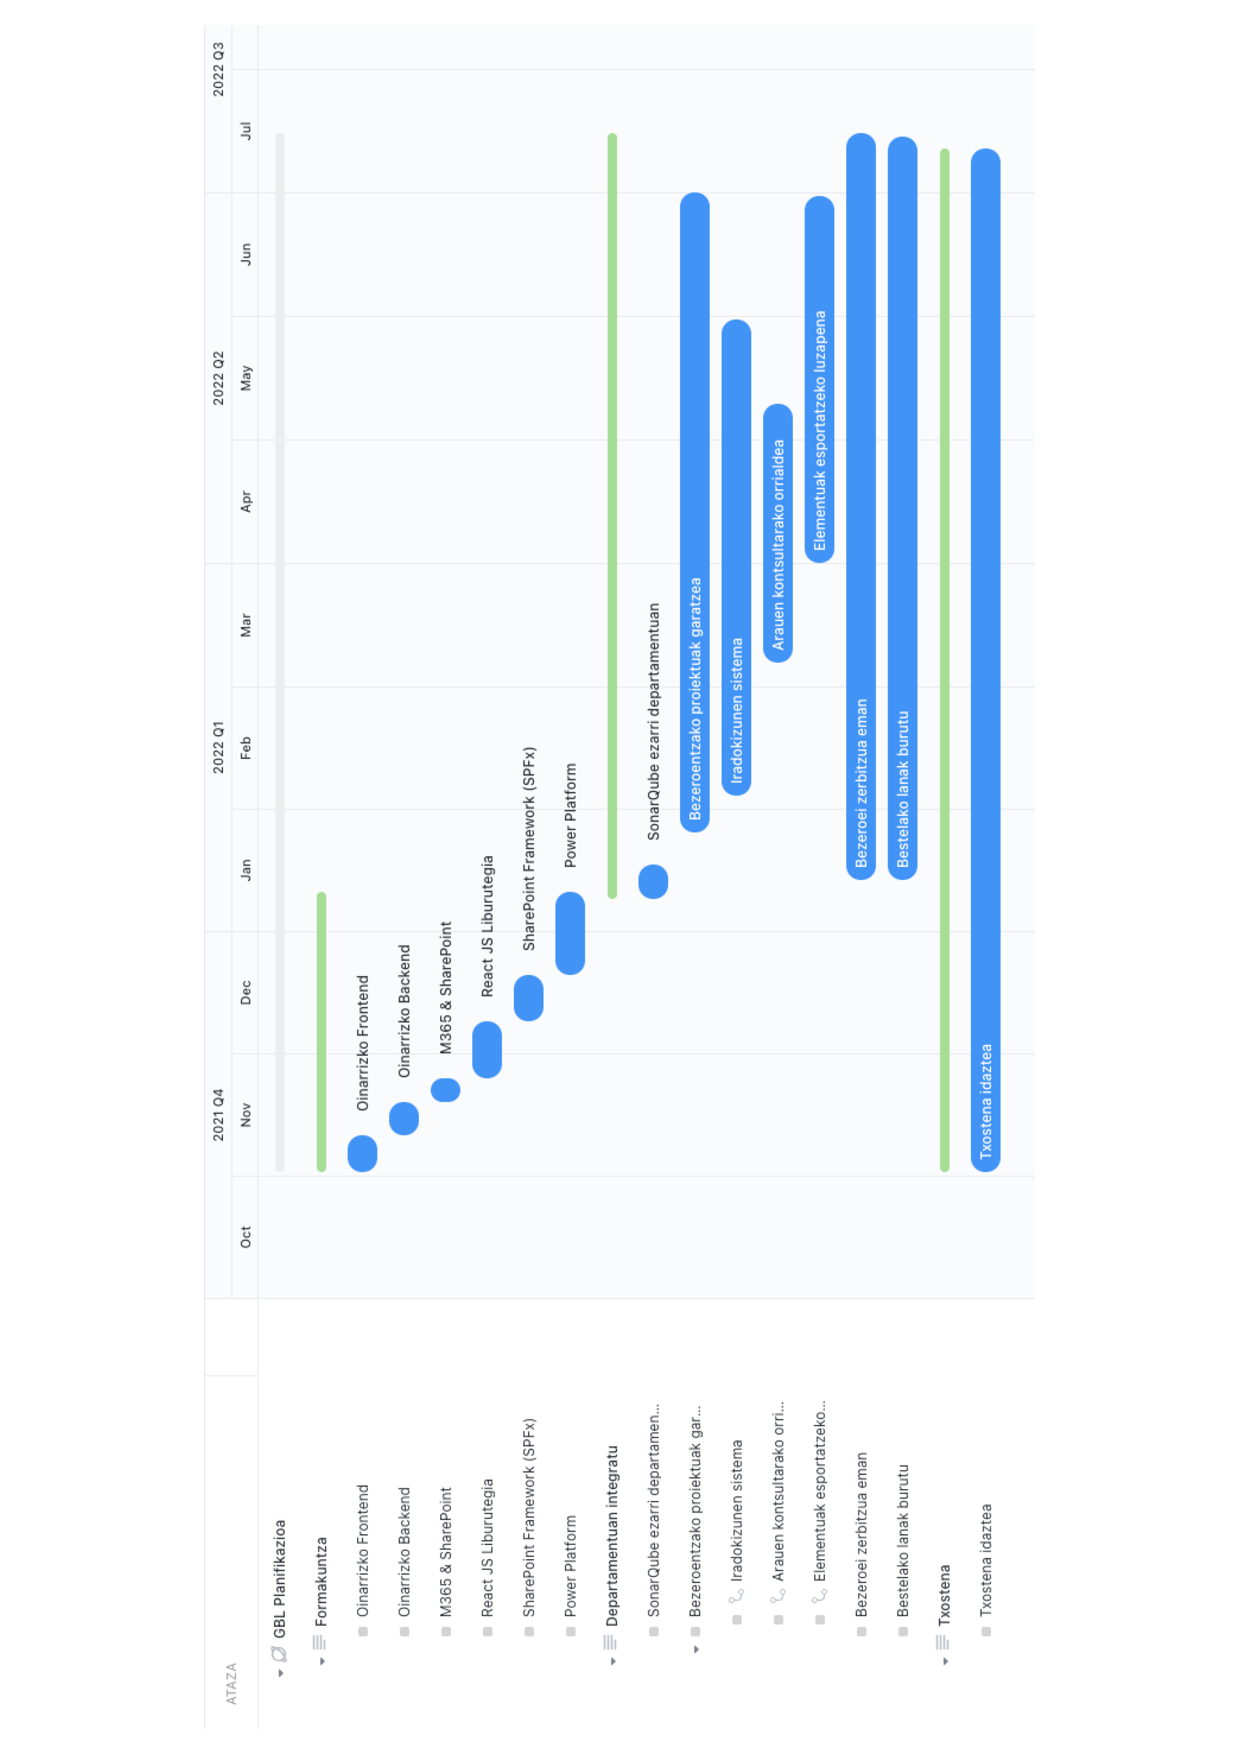
\includepdf[scale=0.75, pages=1, angle=180, pagecommand=\section{Proiektuaren planifikazioaren Gantt diagrama}\label{app:gantt}]{Assets/gantt-final.pdf}

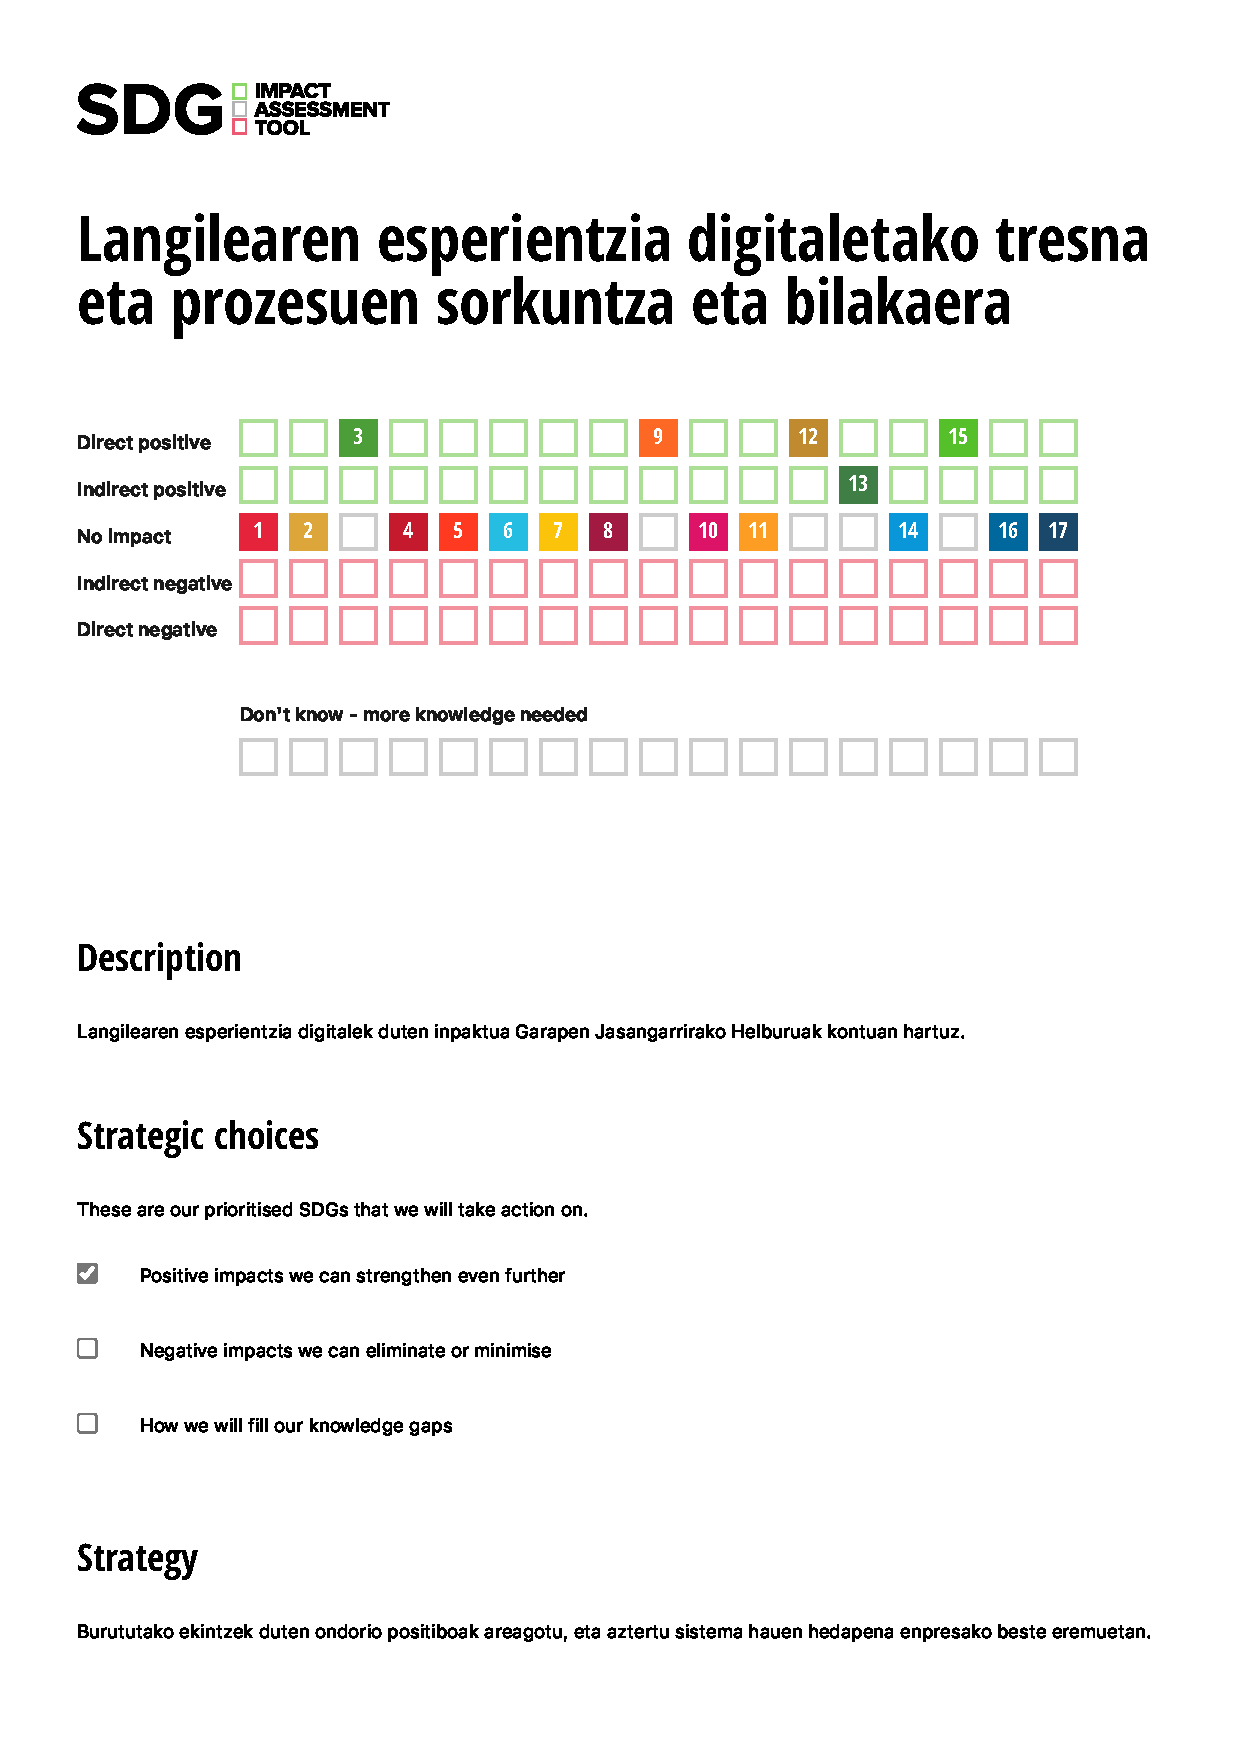
\includepdf[scale=0.75, pages=1,pagecommand=\section{Proiektuaren inpaktua Garapen Jasangarrirako Helburuekiko}\label{app:gjh}]{Assets/sdg-gbl.pdf}
\includepdf[scale=0.80, pages=2-last, pagecommand=\thispagestyle{eranskinak}]{Assets/sdg-gbl.pdf}

\pagestyle{plain}



  \printindex
  \printbibliography

\end{document}
